\documentclass[12pt,a4paper]{report}
\usepackage[
 inner=2.5cm, % Inner margin
	outer=3.8cm, % Outer margin
	bindingoffset=2cm, % Binding offset
	top=1.5cm, % Top margin
	bottom=1.5cm
]{geometry}
\linespread{1.5}

\newcommand\floor[1]{\lfloor#1\rfloor}
\newcommand\ceil[1]{\lceil#1\rceil}
	
\bibliographystyle{apalike}
%\usepackage{algorithm,algpseudocode,float}
%\algrenewcommand\alglinenumber[1]{\tiny #1:}

%\usetikzlibrary{external}
%\tikzset{external/system call={pdflatex \tikzexternalcheckshellescape -halt-on-error
%-interaction=batchmode -jobname "\image" "\texsource" &&
%dvips -o "\image".ps "\image".dvi;
%ps2eps "\image.ps"}}
%\tikzexternalize

\usepackage{enumerate}
\usepackage[font=small,labelfont=bf]{caption}
\usepackage{amsmath,latexsym,amssymb, mathrsfs}
\usepackage{varioref,amssymb,amsthm}
\usepackage{pstricks,graphicx}
%\usepackage{glossaries}
\usepackage{titlesec}
\usepackage{epstopdf}
\usepackage{anysize}
\usepackage{epsfig}
\usepackage{epstopdf}
%\usepackage{algorithm2e}
%\usepackage{algorithmic}
\usepackage{setspace}
\usepackage{enumitem}
\usepackage{subfigure}
\usepackage{array}
\usepackage{longtable}
\renewcommand\arraystretch{1.3} 
\usepackage{enumerate}
\usepackage{varioref,tabularx,longtable,multirow,array,float}
\usepackage{amsmath,latexsym,amssymb,tikz}
\usepackage{varioref,amssymb,amsthm}
\usepackage{mathrsfs}
\usepackage{times}
\usepackage[numbers]{natbib}
\usepackage{color}
\usepackage{graphicx}
\usepackage{indentfirst}
\usepackage{algorithm,algpseudocode,float}
\algrenewcommand\alglinenumber[1]{\tiny #1:}
\usepackage{csquotes}
%\algrenewcommand\algorithmicindent{2.0em}%
%\usepackage{algorithmic}
\usepackage{longtable}

\usepackage{amsfonts}
%\usepackage{endmmacro}
\usepackage{graphicx}
\usepackage{hyperref}
\usepackage{caption}

\usepackage{xpatch}
%\usepackage{subcaption}
%\usepackage{tikz}

%\usetikzlibrary{external}
%\tikzset{external/system call={pdflatex \tikzexternalcheckshellescape -halt-on-error
%-interaction=batchmode -jobname "\image" "\texsource" &&
%dvips -o "\image".ps "\image".dvi;
%ps2eps "\image.ps"}}
%\tikzexternalize

\makeatletter
\xpatchcmd{\algorithmic}{\itemsep\z@}{\itemsep=-1ex plus-1pt}{}{}
\makeatother

\makeatletter
\newenvironment{breakablealgorithm}
  {% \begin{breakablealgorithm}
   \begin{center}
     \refstepcounter{algorithm}% New algorithm
     \hrule height.8pt depth0pt \kern2pt% \@fs@pre for \@fs@ruled
     \renewcommand{\caption}[2][\relax]{% Make a new \caption
       {\raggedright\textbf{\ALG@name~\thealgorithm} ##2\par}%
       \ifx\relax##1\relax % #1 is \relax
         \addcontentsline{loa}{algorithm}{\protect\numberline{\thealgorithm}##2}%
       \else % #1 is not \relax
         \addcontentsline{loa}{algorithm}{\protect\numberline{\thealgorithm}##1}%
       \fi
       \kern2pt\hrule\kern2pt
     }
  }{% \end{breakablealgorithm}
     \kern2pt\hrule\relax% \@fs@post for \@fs@ruled
   \end{center}
  }
\makeatother

\usepackage{tikz}
\newcommand\tikzmark[1]{%
  \tikz[remember picture,overlay]\node[inner sep=2pt] (#1) {};}
\newcommand\DrawBox[3][]{%
  \tikz[remember picture,overlay]\draw[#1] ([xshift=-3.5em,yshift=7pt]#2.north west) rectangle (#3.south east);}

\algnewcommand\algorithmicinput{\textbf{Input:}}
\algnewcommand\INPUT{\item[\algorithmicinput]}

\algnewcommand\algorithmicoutput{\textbf{Output:}}
\algnewcommand\OUTPUT{\item[\algorithmicoutput]}

\titleformat{\section}{\normalsize\bfseries}{\thesection}{1em}{}
\titleformat{\subsection}{\normalsize\bfseries}{\thesubsection}{1em}{}

\titleformat{\chapter}[display]
{\normalfont\large\filcenter\bfseries}
{
\large\MakeUppercase{\chaptertitlename} \thechapter}
{14pt}
{
\large}


\newtheorem{theorem}{Theorem}[section]
\newtheorem{Definition}{Definition}[section]
\newtheorem{proposition}{Proposition}[section]
\newtheorem{corollary}{Corollary}[theorem]
\newtheorem{lemma}[theorem]{Lemma}
\newtheorem{case}{Case}
\newtheorem{subcase}{Case}
\numberwithin{subcase}{case}
\usepackage[utf8]{inputenc}

\begin{document}
\thispagestyle{empty}
\begin{center}
{\normalsize
 {\Large \bf Complexity of Variants of Connected Domination in Graphs \\}

\vspace{1cm}

{\em \bf A thesis submitted in the fulfilment for the requirements of the}
{\em \bf degree of\\ 
{\large \bf Bachelor of Technology\\}}
{in}\\
{\em \bf \large Computer Science and Engineering}

{ by}\\
\vspace*{0.5cm}
{\large{\bf Pratyush Kamal Chaudhary (157148)}}\\
{\large{\bf Avinash Bunde (157108)}}\\
{\large{\bf Rajendra Kujur (157150)}}\\


\vspace*{1cm}
{\bf Under the Guidance of }\\
\vspace*{0.3cm}
{\large{\bf Dr. P. Venkata Subba Reddy}}\\
{\large{\bf Assistant Professor, Department of CSE}}\\
%{\large{\bf Department of CSE,}}\\
{\large{\bf NIT Warangal}}\\

\vspace*{0.3cm}

\vspace*{1.0cm}

\begin{figure}[ht]
\centering
\includegraphics[height=4cm,width=3.5cm]{./images/log_nitw.eps}
\end{figure}

\large{\bf Department of Computer Science and Engineering}\\
\large{
\bf National Institute of Technology\\ Warangal}\\

{\bf 2018-19}
}
\end{center}
\newpage
\pagenumbering{roman}
\setcounter{page}{2}
\vspace*{7.5cm}
\textit{\textbf{
\begin{center}
\LARGE Dedicated To My Parents
\end{center}
}
}
\newpage
\begin{center}
\vspace*{1.00cm}
{\Large\bf Dissertation Approval for B.Tech.}\\
\vspace*{1.00cm}
{\em This Project Work entitled}\\
 {\large \textbf {Roman \{2\}-domination in Graphs}\\}
{by}\\
{\bf Pratyush Kamal Chaudhary}\\
{\bf Avinash Bunde}\\
{\bf Rajendra Kujur}\\
{\em is approved for the Degree of }\\
{\textbf {B. Tech in Computer Science and Engineering}\\}
\vspace*{0.5cm}
{\em \bf Examiners\\}
...........................\\
...........................\\
...........................\\
\vspace*{0.5cm}
{\em \bf Supervisor(s)\\}
............................\\
............................\\
\vspace*{0.5cm}
{\em \bf Chairman\\}
............................\\


\vspace*{1.5cm}
\end{center}
\vspace*{1.5cm}
\large{\textbf{Date:} ..............................} \\
\large{\textbf{Place:} .............................}








\newpage

\begin{center}
{
{\bf \normalsize {DEPARTMENT OF COMPUTER SCIENCE AND ENGINEERING}}\\
{\bf \large NATIONAL INSTITUTE OF TECHNOLOGY}\\
{\bf \large WARANGAL}
} 
\vspace*{2cm}
\begin{figure}[ht]
\centering
\includegraphics[height=4cm,width=3.5cm]{./images/log_nitw.eps}
\end{figure}
\vspace*{1cm}

{\large \bf {CERTIFICATE}}\\
\end{center}
{\normalsize
This is to certify that the project titled \textbf{\enquote{Roman \{2\}-domination in Graphs} } is a bonafide work carried out by {\bf Pratyush Kamal Chaudhary (Roll No. 157148), Avinash Bunde (Roll No. 157112), Rajendra Kujur (Roll No. 157150)} in partial fulfilment of the requirements for the award of the degree of {\bf B.Tech.} in \textbf{Computer Science and Engineering} and submitted to the {Department of Computer Science and Engineering, National Institute of Technology, Warangal}.\\ \\ \\ 

\parbox[t]{55mm}{\bf
Dr. P. Venkata Subba Reddy\\
Project Guide\\
Department of CSE\\NIT Warangal
}
\hfill
\parbox[t]{50mm}
{\bf
Dr. R. B. V. Subramanyam\\
Head of the Department\\
Department of CSE\\
NIT Warangal}
}
\newpage


















\begin{center}
\vspace*{1.00cm}
{\large{\bf DECLARATION }}
\end{center}
{\normalsize
I declare that this written submission represents my ideas in my own words and where
others' ideas or words have been included, I have adequately cited and referenced the
original sources. I also declare that I have adhered to all principles of academic honesty
and integrity and have not misrepresented or fabricated or falsified any idea / data / fact
/ source in my submission. I understand that any violation of the above will be the cause
for disciplinary action by the Institute and can also evoke penal action from the sources
which have thus not been properly cited or from whom proper permission has not been
taken when needed.\\
\noindent
......................................\\
\vspace*{0.2cm}
\textbf{Signature}\\
\vspace*{0.2cm}
\textbf{Pratyush Kamal Chaudhary}\\
\vspace*{0.2cm}
\textbf{Roll no. 157148}\\
\vspace*{0.2cm}
\textbf{Signature}\\
\vspace*{0.2cm}
\textbf{Avinash Bunde}\\
\vspace*{0.2cm}
\textbf{Roll no. 157108}\\
\vspace*{0.2cm}
\textbf{Signature}\\
\vspace*{0.2cm}
\textbf{Rajendra Kujur}\\
\vspace*{0.5cm}
\textbf{Roll no. 157150}\\
\textbf{Date: ...................}\\
}
\newpage

\newpage
\addcontentsline{toc}{chapter}{Abstract}
\bigskip  \bigskip \bigskip \bigskip \bigskip \bigskip
\hfill  \hfill \hfill
\Large
\begin{center}
\textbf{Abstract}
\end{center}
\newcommand{\rdom}{\gamma_{R2}}
\bigskip  
\small
A Roman {2}-dominating function (R2DF) on a graph $G = (V,E)$ is defined as a function $f: V(G) \rightarrow \{0,1,2\}$, which satisfies the condition that for any vertex $u \in V$ having $f(u) = 0$, there is at least one vertex $v$ adjacent to $u$ where $f(v) = 2$ or there are at least two vertices $x$,$y$ adjacent to $u$ where $f(x) = f(y) = 1$.

The weight of a R2DF $f$ is the value $f(V) = \sum_{v \in V} f(v)$.The minimum weight of a R2DF $f$ on a graph G is the Roman {2}-domination number $\rdom(G)$. Finding $\rdom$ for a general graph $G$ is proved to be an NP-complete problem.

In this paper we will begin our discussion with upper bound and exact results obtained for $\rdom$ in some special classes of Graphs. In particular, we present the exact value of $\rdom$ in Square of Cycle Graphs ($C_{n^{2}}$) and Rook's Graph. We also give a tight upper bound of $\rdom$ in King's Graph.

Next we present a linear time dynamic programming algorithm for finding $\rdom(T)$ in a tree $T$.
\\

\textbf{Keywords:} Roman {2}-domination, NP-complete, Square of Graphs, Cycle Graphs, Rook's Graph, King's Graph, dynamic programming, tree.


 
\newpage
\addcontentsline{toc}{chapter}{Acknowledgements}
\bigskip  \bigskip \bigskip \bigskip \bigskip \bigskip
\hfill  \hfill \hfill
\Large
\begin{center}
\textbf{ACKNOWLEDGEMENTS}
\end{center}
\bigskip  
\small
This thesis would not have been possible without the help and cooperation of many. I would like to thank the following people who have helped me directly or indirectly to complete my research work and make this thesis. \par \noindent
First and foremost, I would like to thank my project guide \textbf {Dr. P. Venkata Subba Reddy}, Assistant Prof., Dept. of CSE, NIT Warangal, for constantly guiding and encouraging me throughout the entire duration of my project work. He has not only helped me with his technical knowledge but also with his moral values. He has inspired me with his work ethic and his passion for research work. I could not have completed this work without him.   
\par \noindent
I thank the Ministry of Human Resource Development (MHRD), New Delhi, India, for their financial support during my B. Tech. program. I must also thank all the faculty members in the Dept. of CSE, NIT Warangal for their cooperation during my M. Tech. program.
\par \noindent
I am grateful to the following authors and researchers \textbf{J. Cyman, M. Lemanska, J. Raczek} for introducing the concept of doubly connected domination in graphs \cite{dcds} and \textbf{B. H. Arriola, S. R. Canoy} for introducing the concept of secure doubly connected domination in graphs in \cite{sdcds} and also \textbf{S. V. D. Rashmi, S. Arumugam} for introducing the concept of perfect secure domination in graphs in \cite{pscd}.
\par \noindent
Finally I would like to thank my mother \textbf{Laxmidevi} and my father \textbf{Vijay Narayan Gupta}, for believing in me. This project work would not have been possible without their constant support, love and affection.
\vspace{0.25in}
\begin{flushright}
\textbf{(Deepakkumar Vijay Gupta)}
\end{flushright}
\newpage 
\renewcommand\contentsname{\large \textbf{Table of Contents}}
\addcontentsline{toc}{chapter}{Table of Contents}
\tableofcontents
\newpage
\renewcommand\listfigurename{\large \textbf{List of Figures}}
\addcontentsline{toc}{chapter}{List of Figures}
\listoffigures
\thispagestyle{empty}
\bigskip \bigskip
\newpage
\thispagestyle{empty}
%\bigskip  \bigskip \bigskip \bigskip \bigskip \bigskip
\hfill  \hfill \hfill
\Large
\begin{center}
\textbf{Abstract}
\end{center}
\newcommand{\rdom}{\gamma_{R2}}
\bigskip  
\small
A Roman {2}-dominating function (R2DF) on a graph $G = (V,E)$ is defined as a function $f: V(G) \rightarrow \{0,1,2\}$, which satisfies the condition that for any vertex $u \in V$ having $f(u) = 0$, there is at least one vertex $v$ adjacent to $u$ where $f(v) = 2$ or there are at least two vertices $x$,$y$ adjacent to $u$ where $f(x) = f(y) = 1$.

The weight of a R2DF $f$ is the value $f(V) = \sum_{v \in V} f(v)$.The minimum weight of a R2DF $f$ on a graph G is the Roman {2}-domination number $\rdom(G)$. Finding $\rdom$ for a general graph $G$ is proved to be an NP-complete problem.

In this paper we will begin our discussion with upper bound and exact results obtained for $\rdom$ in some special classes of Graphs. In particular, we present the exact value of $\rdom$ in Square of Cycle Graphs ($C_{n^{2}}$) and Rook's Graph. We also give a tight upper bound of $\rdom$ in King's Graph.

Next we present a linear time dynamic programming algorithm for finding $\rdom(T)$ in a tree $T$.
\\

\textbf{Keywords:} Roman {2}-domination, NP-complete, Square of Graphs, Cycle Graphs, Rook's Graph, King's Graph, dynamic programming, tree.


 
\newpage
\pagenumbering{arabic}
\setcounter{page}{1}
\chapter{Introduction}

\section{Graph Theory and Domination}
Graph theory, a branch of discrete mathematics, is the study of graphs. A graph can be considered as a mathematical structure modelling the pairwise relations between various objects. In a graph, the objects are usually represented by nodes while the relation between them is represented by an edge. 
Formally, a graph is an ordered pair $G = (V,E)$ where $V$ denotes the set of vertices, while $E$ denotes the set of edges, each connecting a pair of vertices. An edge $e \in E$ is an ordered pair $e = (u,v)$ which indicates there is a relation between vertices $u \in V$ and $v \in V$. 
\\
A dominating set of a graph $G$ is the subset $D \subseteq V$ such that for any vertex $u \notin D$, there exists a vertex $v \in D$ which is adjacent to $u$. The minimum size of a dominating set $|D|$ of a graph $G$ is called domination number $\gamma(G)$ of the graph.
\\
\begin{figure}[H]
	\centering
	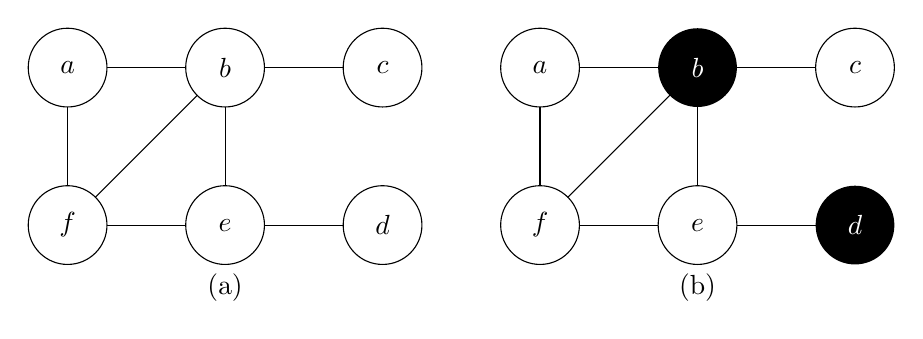
\begin{tikzpicture}
	\draw (0.5,0) -- (1.5,0);
	\draw (2.5,0) -- (3.5,0);
	\draw (0.5,2) -- (1.5,2);
	\draw (2.5,2) -- (3.5,2);
	\draw (0,1.5) -- (0,0.5);
	\draw (0.35,0.35) -- (1.65,1.65);
	\draw (2,1.5) -- (2,0.5);
	
	%\draw (2,2) -- (2,0) -- (0,2);
	
	\draw (0,2) circle(0.5) node{$a$};
	\draw (2,2) circle(0.5) node{$b$};
	\draw (4,2) circle(0.5) node{$c$};
	\draw (4,0) circle(0.5) node{$d$};
	\draw (2,0) circle(0.5) node{$e$};
	\draw (0,0) circle(0.5) node{$f$};
	\draw (2,-0.8) node{(a)};
	
	%-------------------------------------
	\draw (6.5,0) -- (7.5,0);
	\draw (8.5,0) -- (9.5,0);
	\draw (6.5,2) -- (7.5,2);
	\draw (8.5,2) -- (9.5,2);
	\draw (6,1.5) -- (6,0.5);
	\draw (6.35,0.35) -- (7.65,1.65);
	\draw (8,1.5) -- (8,0.5);
	
	%\draw (2,2) -- (2,0) -- (0,2);
	
	\draw (6,2) circle(0.5) node{$a$};
	\fill (8,2) circle(0.5) node[text=white]{$b$};
	\draw (10,2) circle(0.5) node{$c$};
	\fill (10,0) circle(0.5) node[text=white]{$d$};
	\draw (8,0) circle(0.5) node{$e$};
	\draw (6,0) circle(0.5) node{$f$};
	\draw (8,-0.8) node{(b)};
	
	\end{tikzpicture}
	\caption{(a) Graph $G$ (b) Graph $G$ with $\gamma $ set}
\end{figure}
\noindent
In Figure 1.1, the set of vertices $D= \{ b,d\}$ form a minimum dominating set. Note that there can be more than one minimum dominating set for a graph, in Figure 1.3, $\{ b,e \}$ is also a minimum DS. Therefore, $\gamma(G)=2$. \\
\noindent

\section{Historical Background} 
The formal study in graph theory was initiated in 1736, when Leonhard Euler published a paper containing a solution to the famous K{\"{o}}nigsberg bridge problem. He solved the problem by reducing it into graphs, representing lands by vertices and bridges by edges.
\begin{figure}[H]
\centering
\includegraphics[height=6cm,width=10cm]{images/koenisseg.png}
\caption{The K{\"{o}}nigsberg bridge problem}
\end{figure}
The domination problem was first studied around 1862 when de Jaenisch studied the\textit{queen problem}.The queen problem is basically finding the minimum number of queens to place on a $n \times n$ chessboard such that each chess square is covered or dominated by at least one queen.
 \begin{figure}[H]
	\centering
	\includegraphics[height=6cm,width=6cm]{images/Queens.png}
	\caption{The queen problem}
\end{figure}
However, the rigorous study of domination began in 1960s when the term \textit{dominating set} and \textit{domination number} were introduced.

\section{Basic Definition and Terminologies}
\noindent  
Let $G(V,E)$ with $|V|=n$ and $|E(G)|=m$ be a simple, undirected and connected graph. The \textit{open neighborhood} of a vertex $u \in V(G)$ defined as $N_G(u)$= \{$v  | v \in V(G)$ and $(u,v) \in E(G)$\}, similarly the \textit{closed neighborhood} of a vertex $u$ defined as $N_G[u]=N_G(u) \cup \{u\}$. The \textit {degree} of a vertex $u \in V(G)$ is defined as the number of vertices adjacent to $u$ in $G$, hence $d_G(u) = |N_G(u)|$. Specifically, a vertex $u \in V(G)$ is a \textit{pendant vertex} in $G$, if $d_G(u)=1$. The number of pendant vertices in $G$ is denoted by $n_1(G)$. The vertices adjacent to pendant vertex are called a \textit{support vertex}. For a set $S \subseteq V(G)$, let $G[S]$ denote the \textit{subgraph}, \textit{induced by} $S$ in  $G$. Undefined notations and terminology we can refer  \cite{Chartrand,West}.\\
\noindent
A \textit{Dominating Set} (DS) $D$ is a subset of vertices such that  $\forall v \in V(G) \setminus D$, a vertex $u \in D$ exists and $(u,v)\in E(G)$. The \textit{domination number} of $G$ is denoted by $\gamma(G)$ and defined as the minimum cardinality of a dominating set.\\ 

A \textit{Connected Dominating Set} (CDS) $D$ is a subset of vertices such that $D$ is DS of $G$ and $G[D]$ is connected. The \textit{connected domination number} of $G$ is denoted by $\gamma_c(G)$ and defined as the minimum cardinality of a connected dominating set in $G$.\\
\begin{figure}[H]
		\centering
		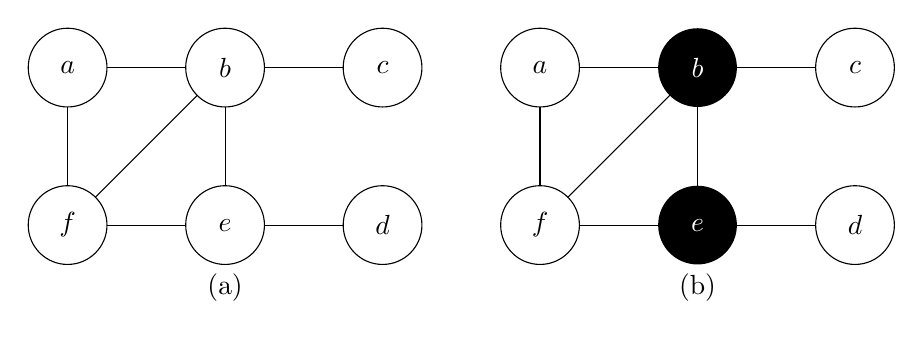
\begin{tikzpicture}
\draw (0.5,0) -- (1.5,0);
\draw (2.5,0) -- (3.5,0);
\draw (0.5,2) -- (1.5,2);
\draw (2.5,2) -- (3.5,2);
\draw (0,1.5) -- (0,0.5);
\draw (0.35,0.35) -- (1.65,1.65);
\draw (2,1.5) -- (2,0.5);

%\draw (2,2) -- (2,0) -- (0,2);

\draw (0,2) circle(0.5) node{$a$};
\draw (2,2) circle(0.5) node{$b$};
\draw (4,2) circle(0.5) node{$c$};
\draw (4,0) circle(0.5) node{$d$};
\draw (2,0) circle(0.5) node{$e$};
\draw (0,0) circle(0.5) node{$f$};
\draw (2,-0.8) node{(a)};

%-------------------------------------
\draw (6.5,0) -- (7.5,0);
\draw (8.5,0) -- (9.5,0);
\draw (6.5,2) -- (7.5,2);
\draw (8.5,2) -- (9.5,2);
\draw (6,1.5) -- (6,0.5);
\draw (6.35,0.35) -- (7.65,1.65);
\draw (8,1.5) -- (8,0.5);

%\draw (2,2) -- (2,0) -- (0,2);

\draw (6,2) circle(0.5) node{$a$};
\fill (8,2) circle(0.5) node[text=white]{$b$};
\draw (10,2) circle(0.5) node{$c$};
\draw (10,0) circle(0.5) node{$d$};
\fill (8,0) circle(0.5) node[text=white]{$e$};
\draw (6,0) circle(0.5) node{$f$};
\draw (8,-0.8) node{(b)};

\end{tikzpicture}
\caption{(a) Graph $G$ (b) Graph $G$ with $\gamma_c$ set}
\end{figure}
\noindent
In Figure 1.4, the set of vertices $D= \{ b,e\}$ form a minimum CDS. Therefore,  $\gamma_c(G)=2$. \\
\noindent
The concept of \textit{doubly connected domination} has been introduced by J. Cyman et al. in \cite{dcds}. A \textit{doubly connected dominating set} (DCDS) $D$ in $G$ is a subset of vertices such that $D$ is a DS of $G$ and $G[V(G)\setminus D]$ and $G[D]$ are connected. The \textit{doubly connected domination number} of $G$ is denoted by $\gamma_{cc}(G)$ and defined as the minimum cardinality of a doubly connected dominating set in $G$.
\begin{figure}[H]
		\centering
		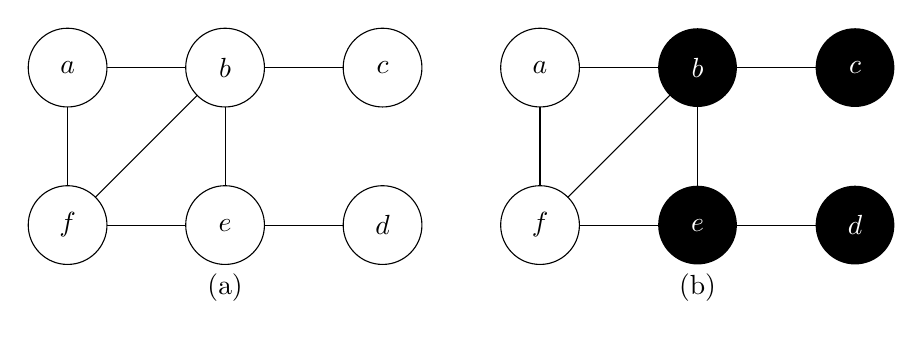
\begin{tikzpicture}
\draw (0.5,0) -- (1.5,0);
\draw (2.5,0) -- (3.5,0);
\draw (0.5,2) -- (1.5,2);
\draw (2.5,2) -- (3.5,2);
\draw (0,1.5) -- (0,0.5);
\draw (0.35,0.35) -- (1.65,1.65);
\draw (2,1.5) -- (2,0.5);

%\draw (2,2) -- (2,0) -- (0,2);

\draw (0,2) circle(0.5) node{$a$};
\draw (2,2) circle(0.5) node{$b$};
\draw (4,2) circle(0.5) node{$c$};
\draw (4,0) circle(0.5) node{$d$};
\draw (2,0) circle(0.5) node{$e$};
\draw (0,0) circle(0.5) node{$f$};
\draw (2,-0.8) node{(a)};

%-------------------------------------
\draw (6.5,0) -- (7.5,0);
\draw (8.5,0) -- (9.5,0);
\draw (6.5,2) -- (7.5,2);
\draw (8.5,2) -- (9.5,2);
\draw (6,1.5) -- (6,0.5);
\draw (6.35,0.35) -- (7.65,1.65);
\draw (8,1.5) -- (8,0.5);

%\draw (2,2) -- (2,0) -- (0,2);

\draw (6,2) circle(0.5) node{$a$};
\fill (8,2) circle(0.5) node[text=white]{$b$};
\fill (10,2) circle(0.5) node[text=white]{$c$};
\fill (10,0) circle(0.5) node[text=white]{$d$};
\fill (8,0) circle(0.5) node[text=white]{$e$};
\draw (6,0) circle(0.5) node{$f$};
\draw (8,-0.8) node{(b)};

\end{tikzpicture}
\caption{(a) Graph $G$ (b) Graph $G$ with $\gamma_{cc}$ set}
\end{figure}
\noindent
In Figure 1.5, the set of vertices $D= \{ b,c,d,e\}$ form a minimum DCDS. Therefore, $\gamma_{cc}(G)=4$. \\
\noindent
E.J. Cockayne et al. has introduced the concept of \textit{secure domination} in \cite{Cockayne}. A \textit{Secure Dominating Set} (SDS) $S$ is a subset of vertices such that for every vertex $v \in V(G) \setminus S$ and a vertex $u \in S$ exists such that there $v$ and $u$ are adjacent and $(S\setminus \{v\}) \cup \{u\}$ is DS of $G$. The \textit{secure domination number}  of $G$ is denoted by $\gamma_s(G)$ and defined as the minimum cardinality of a secure dominating set in $G$.\\
\begin{figure}[H]
		\centering
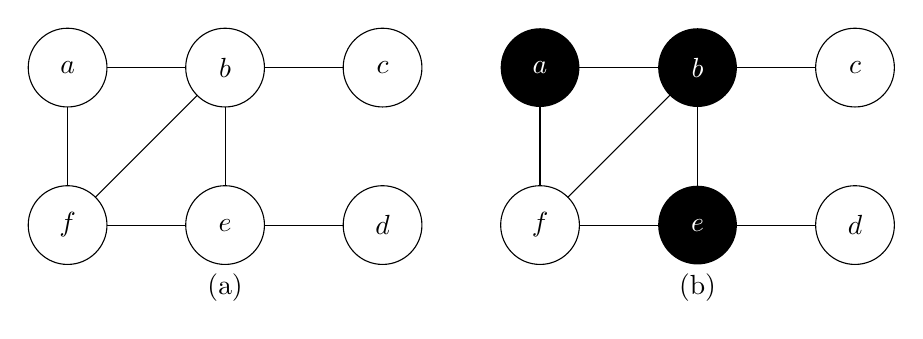
\begin{tikzpicture}
\draw (0.5,0) -- (1.5,0);
\draw (2.5,0) -- (3.5,0);
\draw (0.5,2) -- (1.5,2);
\draw (2.5,2) -- (3.5,2);
\draw (0,1.5) -- (0,0.5);
\draw (0.35,0.35) -- (1.65,1.65);
\draw (2,1.5) -- (2,0.5);

%\draw (2,2) -- (2,0) -- (0,2);

\draw (0,2) circle(0.5) node{$a$};
\draw (2,2) circle(0.5) node{$b$};
\draw (4,2) circle(0.5) node{$c$};
\draw (4,0) circle(0.5) node{$d$};
\draw (2,0) circle(0.5) node{$e$};
\draw (0,0) circle(0.5) node{$f$};
\draw (2,-0.8) node{(a)};

%-------------------------------------
\draw (6.5,0) -- (7.5,0);
\draw (8.5,0) -- (9.5,0);
\draw (6.5,2) -- (7.5,2);
\draw (8.5,2) -- (9.5,2);
\draw (6,1.5) -- (6,0.5);
\draw (6.35,0.35) -- (7.65,1.65);
\draw (8,1.5) -- (8,0.5);

%\draw (2,2) -- (2,0) -- (0,2);


\fill (6,2) circle(0.5) node[text=white]{$a$};
\fill (8,2) circle(0.5) node[text=white]{$b$};
\draw (10,2) circle(0.5) node{$c$};
\draw (10,0) circle(0.5) node{$d$};
\fill (8,0) circle(0.5) node[text=white]{$e$};
\draw (6,0) circle(0.5) node{$f$};

\draw (8,-0.8) node{(b)};
\end{tikzpicture}
\caption{(a) Graph $G$ (b) Graph $G$ with $\gamma_{s}$ set}
\end{figure}
\noindent
In Figure 1.6, the set $S= \{ a,b,e \}$ form a minimum secure dominating set. Therefore, $\gamma_s(G)=3$. \\  
\noindent
The concept of \textit{secure doubly connected domination} has been introduced by B. H. Arriola et al. in \cite{sdcds}. A secure doubly connected dominating set (SDCDS) $S$ in $G$ is a subset of vertices such that $S$ is a DCDS and $\forall v \in S \setminus V(G)$, a vertex $u \in S$ exists where the set $  ( S \setminus \{ u \} ) \cup \{ v \} $ is a DCDS in $G$. The \textit{secure doubly connected domination number} denoted by $\gamma_{scc}(G)$ and defined as the the minimum cardinality of a secure doubly connected dominating set in $G$.
\begin{figure}[H]
		\centering
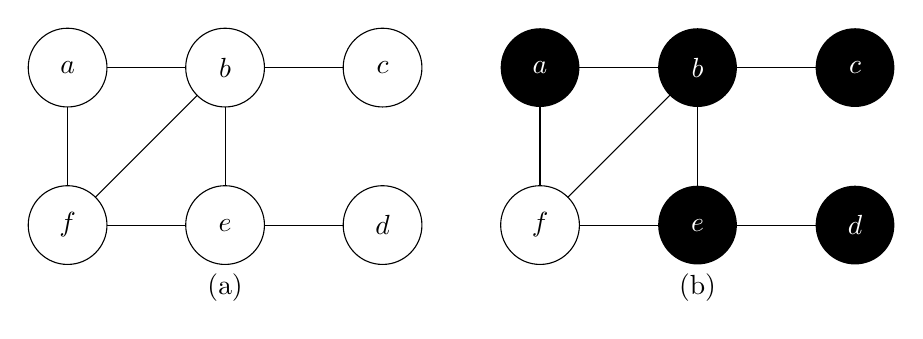
\begin{tikzpicture}
\draw (0.5,0) -- (1.5,0);
\draw (2.5,0) -- (3.5,0);
\draw (0.5,2) -- (1.5,2);
\draw (2.5,2) -- (3.5,2);
\draw (0,1.5) -- (0,0.5);
\draw (0.35,0.35) -- (1.65,1.65);
\draw (2,1.5) -- (2,0.5);

%\draw (2,2) -- (2,0) -- (0,2);

\draw (0,2) circle(0.5) node{$a$};
\draw (2,2) circle(0.5) node{$b$};
\draw (4,2) circle(0.5) node{$c$};
\draw (4,0) circle(0.5) node{$d$};
\draw (2,0) circle(0.5) node{$e$};
\draw (0,0) circle(0.5) node{$f$};
\draw (2,-0.8) node{(a)};

%-------------------------------------
\draw (6.5,0) -- (7.5,0);
\draw (8.5,0) -- (9.5,0);
\draw (6.5,2) -- (7.5,2);
\draw (8.5,2) -- (9.5,2);
\draw (6,1.5) -- (6,0.5);
\draw (6.35,0.35) -- (7.65,1.65);
\draw (8,1.5) -- (8,0.5);

%\draw (2,2) -- (2,0) -- (0,2);

\fill (6,2) circle(0.5) node[text=white]{$a$};
\fill (8,2) circle(0.5) node[text=white]{$b$};
\fill (10,2) circle(0.5) node[text=white]{$c$};
\fill (10,0) circle(0.5) node[text=white]{$d$};
\fill (8,0) circle(0.5) node[text=white]{$e$};
\draw (6,0) circle(0.5) node{$f$};
\draw (8,-0.8) node{(b)};
\end{tikzpicture}
\caption{(a) Graph $G$ (b) Graph $G$ with $\gamma_{scc}$ set}
\end{figure}
\noindent
In Figure 1.7, the set of vertices $S= \{ d,e e,a,b,c \}$ form a minimum secure doubly connected dominating set. Therefore $\gamma_{scc}(G)=5$. \\ 
\noindent
Weichsel has introduced the concept of perfect domination in \cite{Weichsel}. A \textit{Perfect Dominating Set} (PCD) $D$ is a subset of vertices such that  $\forall v \in V(G) \setminus D$, a unique vertex $u \in D$ exists where $u$ and $v$ are adjacent. The \textit{perfect domination number}  of $G$ is denoted by $\gamma_p(G)$ and the minimum cardinality of a perfect dominating set in $G$.\\
\begin{figure}[H]
		\centering
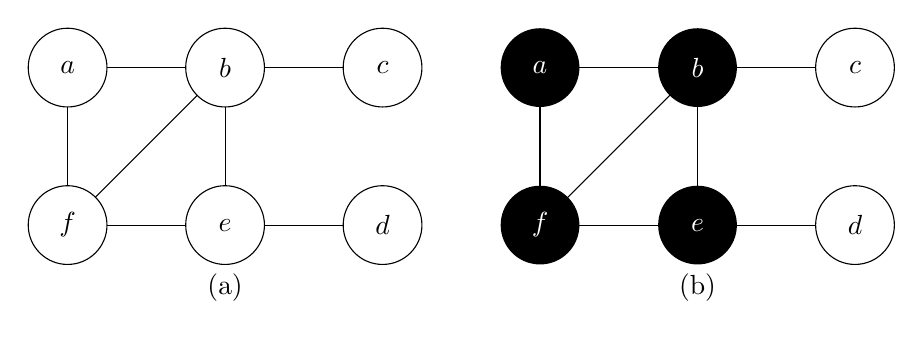
\begin{tikzpicture}
\draw (0.5,0) -- (1.5,0);
\draw (2.5,0) -- (3.5,0);
\draw (0.5,2) -- (1.5,2);
\draw (2.5,2) -- (3.5,2);
\draw (0,1.5) -- (0,0.5);
\draw (0.35,0.35) -- (1.65,1.65);
\draw (2,1.5) -- (2,0.5);

%\draw (2,2) -- (2,0) -- (0,2);

\draw (0,2) circle(0.5) node{$a$};
\draw (2,2) circle(0.5) node{$b$};
\draw (4,2) circle(0.5) node{$c$};
\draw (4,0) circle(0.5) node{$d$};
\draw (2,0) circle(0.5) node{$e$};
\draw (0,0) circle(0.5) node{$f$};
\draw (2,-0.8) node{(a)};

%-------------------------------------
\draw (6.5,0) -- (7.5,0);
\draw (8.5,0) -- (9.5,0);
\draw (6.5,2) -- (7.5,2);
\draw (8.5,2) -- (9.5,2);
\draw (6,1.5) -- (6,0.5);
\draw (6.35,0.35) -- (7.65,1.65);
\draw (8,1.5) -- (8,0.5);

%\draw (2,2) -- (2,0) -- (0,2);

\fill (6,2) circle(0.5) node[text=white]{$a$};
\fill (8,2) circle(0.5) node[text=white]{$b$};
\draw (10,2) circle(0.5) node{$c$};
\draw (10,0) circle(0.5) node{$d$};
\fill (8,0) circle(0.5) node[text=white]{$e$};
\fill (6,0) circle(0.5) node[text=white]{$f$};
\draw (8,-0.8) node{(b)};
\end{tikzpicture}
\caption{(a) Graph $G$ (b) Graph $G$ with $\gamma_p$ set}
\end{figure}
\noindent
In Figure 1.8, the set $D= \{ b,e,f,a \}$ form a minimum perfect dominating set. Therefore, $\gamma_p(G)=4$. \\ 
\noindent
We initiated the study of a variant of secure domination, namely, \textit{secure perfect connected domination}. A { \textit{secure perfect connected dominating set} (SPCDS)} $S$ is a subset of vertices where $G[S]$ is connected and for each vertex $v \in V(G)\setminus S$, a unique vertex $u \in S$ exists such that $u$ and $v$ are adjacent and the set obtained $(S\setminus \lbrace u \rbrace) \cup \lbrace v \rbrace$ is a CDS of $G$. The {\textit{secure perfect connected domination number}} is denoted by {$\gamma_{spc}(G)$} and defined as the minimum cardinality of a SPCDS in $G$.
\begin{figure}[H]
		\centering
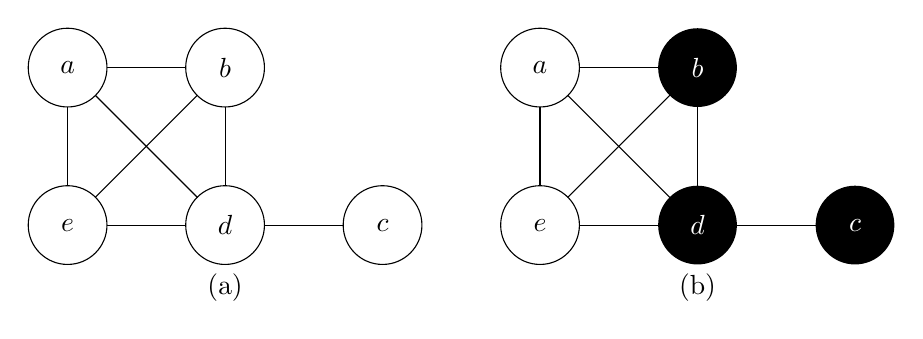
\begin{tikzpicture}
\draw (0.5,0) -- (1.5,0);
\draw (2.5,0) -- (3.5,0);
\draw (0.5,2) -- (1.5,2);
%\draw (2.5,2) -- (3.5,2);
\draw (0,1.5) -- (0,0.5);
\draw (0.35,0.35) -- (1.65,1.65);
\draw (0.35,1.65) -- (1.65,0.35);
\draw (2,1.5) -- (2,0.5);

%\draw (2,2) -- (2,0) -- (0,2);

\draw (0,2) circle(0.5) node{$a$};
\draw (2,2) circle(0.5) node{$b$};
%\draw (4,2) circle(0.5) node{$c$};
\draw (4,0) circle(0.5) node{$c$};
\draw (2,0) circle(0.5) node{$d$};
\draw (0,0) circle(0.5) node{$e$};
\draw (2,-0.8) node{(a)};

%-------------------------------------
\draw (6.5,0) -- (7.5,0);
\draw (8.5,0) -- (9.5,0);
\draw (6.5,2) -- (7.5,2);
%\draw (8.5,2) -- (9.5,2);
\draw (6,1.5) -- (6,0.5);
\draw (6.35,0.35) -- (7.65,1.65);
\draw (6.35,1.65) -- (7.65,0.35);
\draw (8,1.5) -- (8,0.5);

%\draw (2,2) -- (2,0) -- (0,2);

\draw (6,2) circle(0.5) node{$a$};
\fill (8,2) circle(0.5) node[text=white]{$b$};
%\draw (10,2) circle(0.5) node{$c$};
\fill (10,0) circle(0.5) node[text=white]{$c$};
\fill (8,0) circle(0.5) node[text=white]{$d$};
\draw (6,0) circle(0.5) node{$e$};
\draw (8,-0.8) node{(b)};
\end{tikzpicture}
\caption{(a) Graph $G$ (b) Graph $G$ with $\gamma_{spc}$ set}
\end{figure}
\noindent
In Figure 1.9, the set of vertices $S=\{ b,c,d \}$ form a minimum secure perfect connected dominating set. Therefore, $\gamma_{spc}(G)=3$.
\section{Applications of Domination and its Variants}
\subsection{Radio Station}
\noindent
Suppose we need to install a radio station in remote part of the world which has a collection of villages. The radio stations are installed to broadcast the messages to all the villages in the region. Since, radio stations are costly and have limited broadcasting range, we want to install as few radio stations as possible such that messages can be broadcasted to all the villages. We can represent this problem into graph where vertex represents the village and edge represents the distance between two villages. Figure 1.10 shows the representation of village as a graph.
\begin{figure}[H]
\centering
\includegraphics[height=6cm,width=8cm]{images/Village1.png}
    \caption{The collection of villages with distance }
\end{figure}
\noindent
Suppose we are provided the broadcasting range of each radio station then our problem simplifies as to determine the minimum number of radio stations needed such that it dominates all other vertices in graph. First we remove the edges which are more than $50$ km because we have assumed that the broadcasting range of each radio station is not more than $50$ km. Now the problem is reduced to dominating problem and we can easily find the dominating set in the modified graph. Figure 1.11 show the village and its distance only in the range of $50$ km. 
\begin{figure}[H]
\centering
\includegraphics[height=6cm,width=7cm]{images/Village2.png}
    \caption{The collection of villages with distance less than $50$ km}
\end{figure}
\noindent
We can clearly observe that a set $D=\{B, F,H,J\}$ is sufficient to dominate remaining vertices. Thus we can install the radio station at these four places. If we have provided better range of radio station then we may require even less than $4$ radio stations.
\subsection{Bus Routing}
\noindent
In every city many people are traveling by buses. But these buses are having fixed route from one place to other. The organization which manage and decides bus routes, needs to take care that every city must be reachable. Also the nearest bus stop station should be within walkable distance from their current location. There are no bus ride that takes more than some specified number of minutes and limits on the number of passengers that a bus can carry at any one time. Following figure 1.12 represents the street map of a part of city. 
\begin{figure}[H]
\centering
\includegraphics[height=6cm,width=8cm]{images/SchoolBus.png}	
    \caption{Street map of a part of city}
\end{figure}
\noindent
In the above graph edges represents the streets in the city. Now bus organization can decide the bus route such that each passenger can reach to bus stop point by walking at max one block. Thus we can find dominating set such that each block are either a part of bus route or it is a neighbor of the block which are in route. In the above figure the dark line represents the bus route and clearly other vertices not covered in bus route are walkable by at max one block.
\section{Graph Classes}
\subsection{Bipartite Graphs}
\noindent
A graph $G(V_1,V_2,E)$ whose vertex set can be divided into two disjoint independent sets $V_1$ and $V_2$ is called a bipartite graph. A bipartite graph does not have any cycles of odd length. 
\begin{figure}[H]
		\centering
		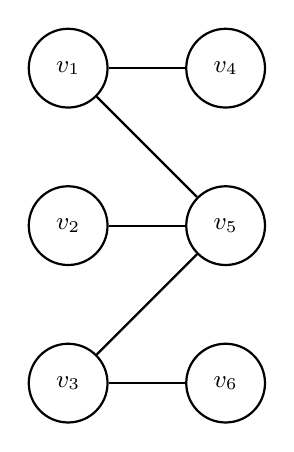
\begin{tikzpicture}[auto, node distance=2.0cm, every loop/.style={}, 
		thick,main node/.style={circle,draw,minimum size=1.0cm,font=\sffamily\small\bfseries}]
			
			\node[main node]  (1) {$v_1$};
			\node[main node] (2) [below of=1] {$v_2$};
			\node[main node] (3) [below of=2] {$v_3$};
			\node[main node] (4) [right of=1] {$v_4$};
			\node[main node] (5) [below of=4] {$v_5$};
			\node[main node] (6) [below of=5]{$v_6$};
			
			
				
			\path[every node/.style={font=\sffamily\small}]
			(1)
			edge node[left] {} (4)
			edge node[left] {} (5)			
									
			(2)
			edge node[left] {} (5)
						
			(3)  
			edge node[left] {} (5)
			edge node[left] {} (6)
			
			;
			\end{tikzpicture}
			\caption{Bipartite graph $G$}
			%\hfill
		\end{figure}
\noindent
Figure 1.13 shows a bipartite graph with $V_1$,$V_2$ being the partite sets. Where $V_1= \{ v_1,v_2,v_3 \}$ and $V_2= \{ v_4,v_5,v_6 \}$. Vertex sets $V_1$ and $V_2$ are independent set.

\subsection{Chordal Graphs}
\noindent
A graph $G(V,E)$ whose all cycles having length four or more in $G$ have a chord is said to be a \textit{chordal graph}. An edge is a chord which is not part of the cycle but connects two vertices of the cycle. 
\begin{figure}[H]
\centering
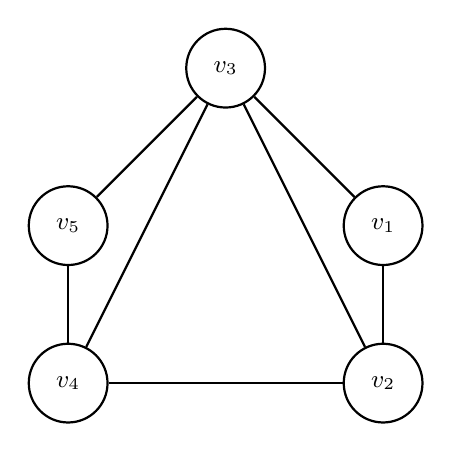
\begin{tikzpicture}[auto, node distance=2.0cm, every loop/.style={},
                    thick,main node/.style={circle,draw,minimum size=1.0cm,font=\sffamily\small\bfseries}]

   \node[main node] (1) {$v_3$};
  \node[main node] (2) [left of=1, below of=1] {$v_5$};
  \node[main node] (3) [right of=1, below of=1] {$v_1$};
  \node[main node] (4) [below of=2] {$v_4$};
  \node[main node] (5) [below of=3] {$v_2$};
  %\node[main node] (6) [below of=5] {};
 


  \path[every node/.style={font=\sffamily\small}]
    (1) %edge node[left] {} (4)
       edge node[left] {} (2)
        edge node[left] {} (3)
        edge node[left] {} (4)
        edge node[left] {} (5)
 
       
    (2) edge node[left] {} (4)
       
       
        
    (3) edge node[left] {}	(5)
    	
    (4)
    	edge node[left] {} (5)
     	
  
     (5)
     
    
       ;
       
\end{tikzpicture}
\caption{Chordal graph $G$}
\end{figure}
\noindent
Figure 1.14 the set $ \{ v_1,v_2,v_4,v_5,v_3\}$ is a cycle and $\{ v_2,v_3\}$, $\{ v_3,v_4\}$ is a chord.


\subsection{Split Graphs}
\noindent
A graph $G(V,E)$ such that whose vertex set $V(G)$ can be partitioned into two disjoint sets $V_1$ and $V_2$ where a clique is formed with vertex set $V_1$ and vertices in $V_2$ form an independent set is said to be a \textit{split graph}. Split graphs is a chordal graphs. \\ \smallskip

\begin{figure}[H]
\centering
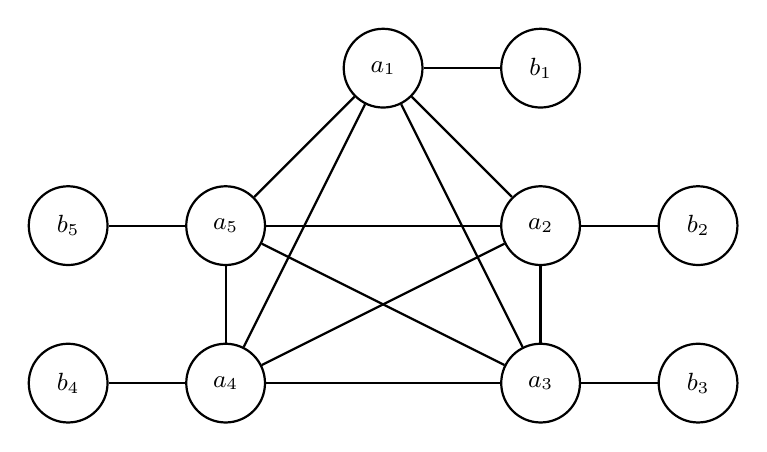
\begin{tikzpicture}[auto, node distance=2.0cm, every loop/.style={},
                    thick,main node/.style={circle,draw,minimum size=1.0cm,font=\sffamily\small\bfseries}]

   \node[main node] (1) {$a_1$};
  \node[main node] (2) [right of=1, below of=1] {$a_2$};
  \node[main node] (3) [below of=2] {$a_3$};
  \node[main node] (5) [left of=1, below of=1] {$a_5$};
  \node[main node] (4) [below of=5] {$a_4$};
  \node[main node] (6) [right of=1] {$b_1$};
  \node[main node] (7) [right of=2] {$b_2$};
  \node[main node] (8) [right of=3] {$b_3$};
  \node[main node] (9) [left of=4] {$b_4$};
  \node[main node] (10) [left of=5] {$b_5$};
 


  \path[every node/.style={font=\sffamily\small}]
    (1) %edge node[left] {} (4)
       edge node[left] {} (2)
        edge node[left] {} (3)
        edge node[left] {} (4)
        edge node[left] {} (5)
        edge node[left] {} (6)
 
       
    (2) edge node[left] {} (3)
    	edge node[left] {} (4)
    	edge node[left] {} (5)
    	edge node[left] {} (7)
       
       
        
    (3) edge node[left] {}	(4)
    	edge node[left] {} (5)
    	edge node[left] {} (8)
    	
    (4)
    	edge node[left] {} (5)
    	edge node[left] {} (9)
     	
  
     (5)
     	edge node[left] {} (10)
    
       ;
       
\end{tikzpicture}
\caption{Split graph $G$}
\end{figure}

\noindent 
Figure 1.15 shows a split graph where $V_1= \{ a_1,a_2,a_3,a_4,a_5 \}$ is a clique and $V_2= \{ b_1,b_2,b_3,b_4,b_5 \}$ is an independent set.

\subsection{Chordal Bipartite Graphs}
\noindent
A bipartite graph $G$ in which every cycle of having length greater than 4 has a chord is a chordal bipartite graph\cite{Brand1}. \\ \smallskip

\begin{figure}[H]
\centering
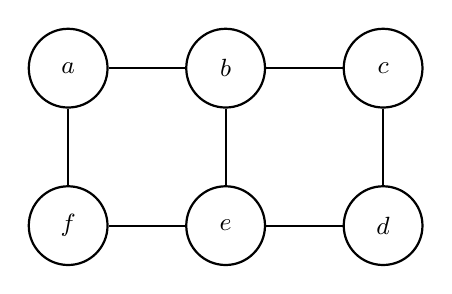
\begin{tikzpicture}[auto, node distance=2.0cm, every loop/.style={},
                    thick,main node/.style={circle,draw,minimum size=1.0cm, font=\sffamily\small\bfseries}]

   \node[main node] (1) {$a$};
  \node[main node] (2) [right of=1] {$b$};
  \node[main node] (3) [right of=2] {$c$};
  \node[main node] (4) [below of=3] {$d$};
  \node[main node] (5) [left of=4] {$e$};
  \node[main node] (6) [left of=5] {$f$};


  \path[every node/.style={font=\sffamily\small}]
    (1) %edge node[left] {} (4)
       edge node[left] {} (2)
        edge node[left] {} (6)
    
       
    (2) edge node[left] {} (3)
    	edge node[left] {} (5)
       
       
        
    (3) edge node[left] {}	(4)
    	
    	
    (4)
    	edge node[left] {} (5)
    	
     	
  
     (5)
     	edge node[left] {} (6)
    
       ;
       
\end{tikzpicture}
\caption{Chordal Bipartite graph $G$}
\end{figure}

\noindent 
Figure 1.16 the set $ \{ a,b,c,d,e,f \}$ is a cycle and $\{ b,c\}$ is a chord.

\subsection{Star Convex Bipartite Graphs}
\noindent
A bipartite graph $G(X,Y,E)$ is a star convex bipartite graph if there is a star $T=(X,F)$ on $X$ such that all vertices of $Y$, its closed neighborhood induces a subtree of $T$ \cite{jiang}. \\ \smallskip

\begin{figure}[H]
		\centering
		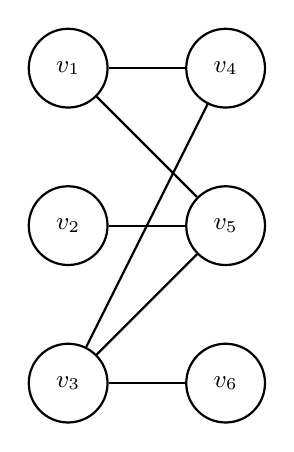
\begin{tikzpicture}[auto, node distance=2.0cm, every loop/.style={}, 
		thick,main node/.style={circle,draw,minimum size=1.0cm,font=\sffamily\small\bfseries}]
			
			\node[main node]  (1) {$v_1$};
			\node[main node] (2) [below of=1] {$v_2$};
			\node[main node] (3) [below of=2] {$v_3$};
			\node[main node] (4) [right of=1] {$v_4$};
			\node[main node] (5) [below of=4] {$v_5$};
			\node[main node] (6) [below of=5]{$v_6$};
			
			
				
			\path[every node/.style={font=\sffamily\small}]
			(1)
			edge node[left] {} (4)
			edge node[left] {} (5)			
									
			(2)
			edge node[left] {} (5)
						
			(3)  
			edge node[left] {} (5)
			edge node[left] {} (6)
			edge node[left] {} (4)			
			
			;
			\end{tikzpicture}
			\caption{Star Convex Bipartite graph $G$}
			%\hfill
		\end{figure}
\noindent
In Figure 1.17, assume tree(star) is formed with vertex set $T= \{ v_1,v_2,v_3\}$ with $v_3$ center vertex then for any vertex from $\{ v_4,v_5, v_6 \}$ its open neighborhood vertex set forms an induce subtree of $T$.

\subsection{Wheel Graphs}
\noindent
A \textit{Wheel graph} denoted by $W_n$ of order $n$ is $K_1 + C_{n-1}$, where $C_{n-1}$ is a cycle of $n-1$ vertices. \\ \smallskip
\begin{figure}[H]
\centering
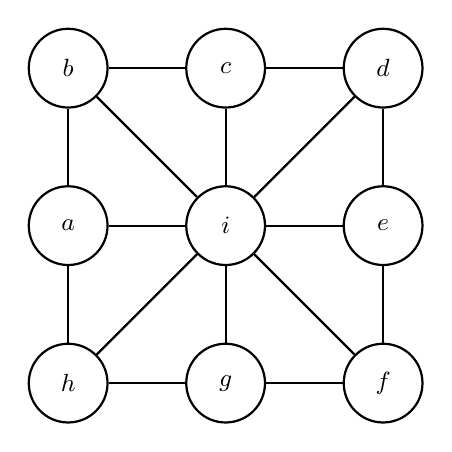
\begin{tikzpicture}[auto, node distance=2.0cm, every loop/.style={},
                    thick,main node/.style={circle,draw,minimum size=1.0cm,font=\sffamily\small\bfseries}]

   \node[main node] (1) {$a$};
   \node[main node] (9) [right of=1]{$i$};
   \node[main node] (5) [right of=9]{$e$};
   \node[main node] (3) [above of=9]{$c$};
   \node[main node] (7) [below of=9]{$g$};
   \node[main node] (2) [above of=1]{$b$};
   \node[main node] (8) [below of=1]{$h$};
   \node[main node] (4) [above of=5]{$d$};
   \node[main node] (6) [below of=5]{$f$};

                        
  


  \path[every node/.style={font=\sffamily\small}]
    (1) %edge node[left] {} (4)
       edge node[left] {} (2)
       
 
       
    (2) edge node[left] {} (3)
    	
       
       
        
    (3) edge node[left] {}	(4)
    	
    (4)
    	edge node[left] {} (5)
    	
     	
  
     (5)
     	edge node[left] {} (6)

     (6)
     	edge node[left] {} (7)
     	(7)
     	edge node[left] {} (8)
     	(8)
     	edge node[left] {} (1)
     (9)
     	edge node[left] {} (1)
     	edge node[left] {} (2)
     	edge node[left] {} (3)
     	edge node[left] {} (4)
     	edge node[left] {} (5)
     	edge node[left] {} (6)
     	edge node[left] {} (7)
     	edge node[left] {} (8)     	

     	    
       ;
       
\end{tikzpicture}
\caption{Wheel graph $W_n$}
\end{figure}

\noindent 
In Figure 1.18, the vertex set $\{ a,b,c,d,e,f,g,h \}$ is a cycle and vertex $\{ i\}$ is common vertex adjacent to all vertices in $W_n$.

\subsection{Fan Graphs}
\noindent
A \textit{Fan graph} $F_n$ is the \textit{join} of $K_1$ with path on $n-1$ vertices i.e. $P_{n-1}$. \\ \smallskip

\begin{figure}[H]
\centering
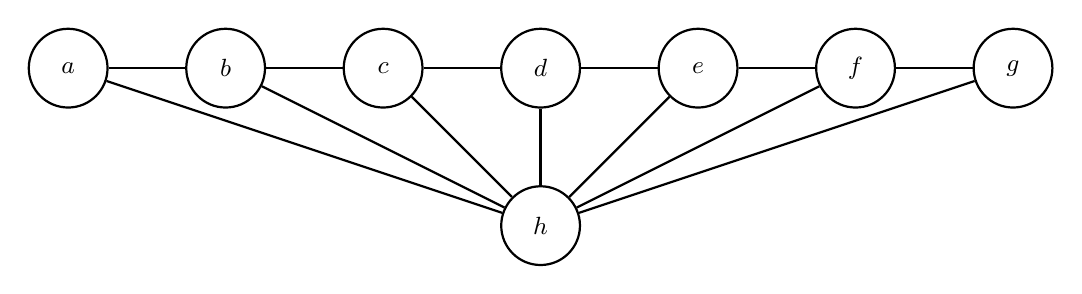
\begin{tikzpicture}[auto, node distance=2.0cm, every loop/.style={},
                    thick,main node/.style={circle,draw,minimum size=1.0cm,font=\sffamily\small\bfseries}]

   \node[main node] (1) {$a$};
   \node[main node] (2) [right of=1]{$b$};
   \node[main node] (3) [right of=2]{$c$};
   \node[main node] (4) [right of=3]{$d$};
   \node[main node] (5) [right of=4]{$e$};
   \node[main node] (6) [right of=5]{$f$};
   \node[main node] (7) [right of=6]{$g$};
   \node[main node] (8) [below of=4]{$h$};
                        
  


  \path[every node/.style={font=\sffamily\small}]
    (1) %edge node[left] {} (4)
       edge node[left] {} (2)
       
 
       
    (2) edge node[left] {} (3)
    	
       
       
        
    (3) edge node[left] {}	(4)
    	
    (4)
    	edge node[left] {} (5)
    	
     	
  
     (5)
     	edge node[left] {} (6)

     (6)
     	edge node[left] {} (7)
     (8)
     	edge node[left] {} (1)
     	edge node[left] {} (2)
     	edge node[left] {} (3)
     	edge node[left] {} (4)
     	edge node[left] {} (5)
     	edge node[left] {} (6)
     	edge node[left] {} (7)

     	    
       ;
       
\end{tikzpicture}
\caption{Fan graph $F_n$}
\end{figure}

\noindent 
In Figure 1.19, the vertex set $\{ a,b,c,d,e,f,g \}$ is a path and vertex $\{ h\}$ is common vertex adjacent to all vertices in $F_n$.

\subsection{Windmill Graphs}
\noindent
The \textit{Windmill graph} denoted by $Wd_{k,n}$ consists of $n$ copies of $K_k$ and identifying one vertex from each $K_k$ copy as a common center vertex. \\ \smallskip

\begin{figure}[H]
\centering
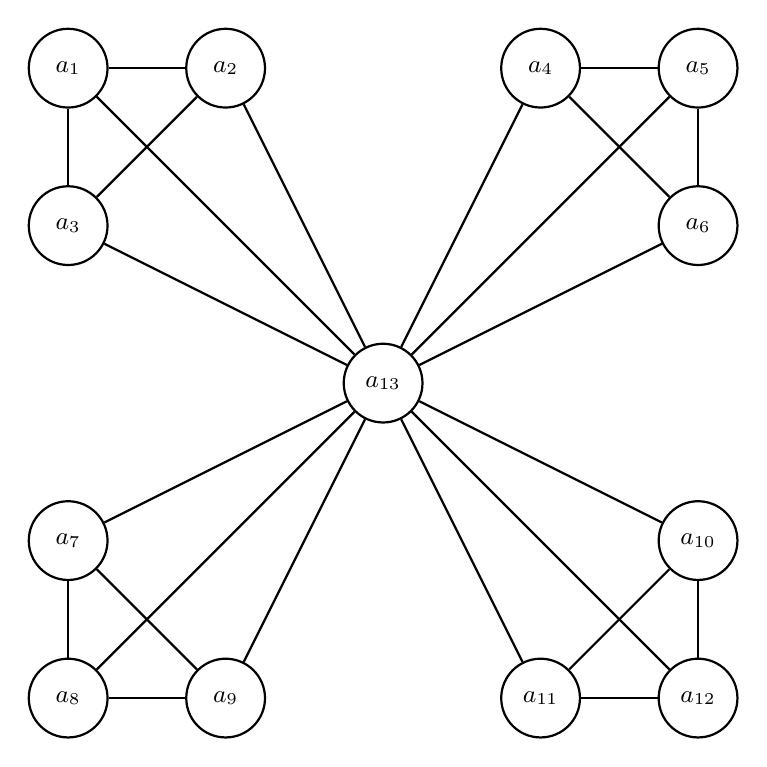
\begin{tikzpicture}[auto, node distance=2.0cm, every loop/.style={},
                    thick,main node/.style={circle,draw,minimum size=1.0cm,font=\sffamily\small\bfseries}]

	\node[main node] (1) {$a_{1}$};
	\node[main node] (2) [right of=1]{$a_{2}$};
	\node (3) [right of=2]{};
	\node[main node] (4) [right of=3]{$a_{4}$};
	\node[main node] (5) [right of=4]{$a_{5}$};
	
	\node[main node] (6) [below of=1]{$a_{3}$};;
	\node (7) [right of=6]{};
	\node (8) [right of=7]{};
	\node (9) [right of=8]{};
	\node[main node] (10) [right of=9]{$a_{6}$};
	
	\node (11) [below of=6]{};
	\node (12) [right of=11]{};
	\node[main node] (13) [right of=12]{$a_{13}$};
	\node (14) [right of=13]{};
	\node (15) [right of=14]{};
	
	\node[main node] (16) [below of=11]{$a_{7}$};;
	\node (17) [right of=16]{};
	\node (18) [right of=17]{};
	\node (19) [right of=18]{};
	\node[main node] (20) [right of=19]{$a_{10}$};
	
	\node[main node] (21) [below of=16]{$a_{8}$};;
	\node[main node] (22) [right of=21]{$a_{9}$};
	\node (23) [right of=22]{};
	\node[main node] (24) [right of=23]{$a_{11}$};
	\node[main node] (25) [right of=24]{$a_{12}$};

  \path[every node/.style={font=\sffamily\small}]
    (1) %edge node[left] {} (4)
       edge node[left] {} (2)
       edge node[left] {} (6)
       
    (2) edge node[left] {} (6)
    	
    (4) edge node[left] {}	(5)
    edge node[left] {}	(10)
    	
    (5)
    	edge node[left] {} (10)
    	
     (16)
     	edge node[left] {} (21)
     	edge node[left] {} (22)

     (21)
     	edge node[left] {} (22)
     	(24)
     	edge node[left] {} (25)
     	edge node[left] {} (20)     	
     	(25)
     	edge node[left] {} (20)
     (13)
     	edge node[left] {} (1)
     	edge node[left] {} (2)
     	edge node[left] {} (4)
     	edge node[left] {} (5)
     	edge node[left] {} (6)
     	edge node[left] {} (10)
     	edge node[left] {} (16)
     	edge node[left] {} (20)
     	edge node[left] {} (21)
     	edge node[left] {} (22)
     	edge node[left] {} (24)
     	edge node[left] {} (25)     	    
       ;
       
\end{tikzpicture}
\caption{Windmill graph $Wd_{k,n}$}
\end{figure}

\noindent 
In Figure 1.20, the vertex sets $\{a_1,a_2,a_3,a_{13}\}$, $\{a_4,a_5,a_6,a_{13}\}$, $\{a_7,a_8,a_9,a_{13}\}$ and $\{a_{10},a_{11},a_{12},a_{13}\}$ are a complete graph $K_4$ and each complete graph shares a common vertex $\{ a_{13}\}$.

\subsection{Trees}
\noindent
A \textit{tree} is an acyclic graph in which there is exactly one path between any two vertices. A tree is always minimally connected, i.e. if an edge is removed from a tree then it becomes a disconnected graph. Let $T(V,E)$ be a tree, where $n$ is the number of vertices, the number of edges is always $n-1$. In a rooted tree, one vertex is designated to be the root. The root has no parent. Non root nodes of degree one are known as leaf nodes, other non root nodes are known as internal nodes.\\
\noindent
Figure 1.21 shows a tree rooted at $v_1$. By $parent(u)$, we denote the parent of vertex $u$. For example, Figure 1.21., $parent(v_2)= v_1$. Similarly, all the children of vertex $v$ are denoted by $children(v)$. For example, in Figure 1.21., $children(v_2)=\{ v_4,v_5 \}$.
\begin{figure}[H]
		\centering
		%\begin{subfigure}%{1\textwidth}
			%\centering
			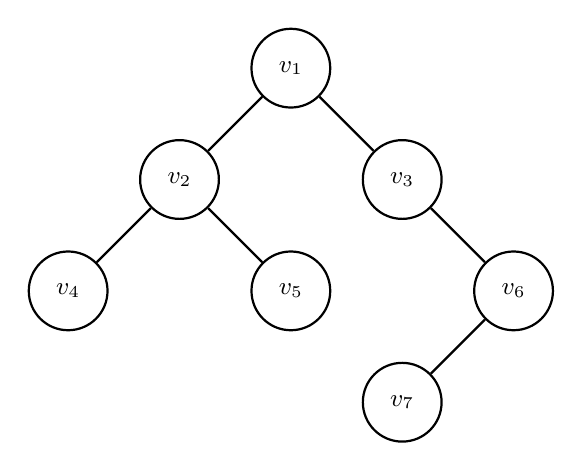
\begin{tikzpicture}[auto, node distance=2.0cm, every loop/.style={},
			thick,main node/.style={circle,draw,minimum size=1.0cm,font=\sffamily\small\bfseries}]
			
			\node[main node] (1) {$v_1$};
			\node[main node] (2) [below left of=1] {$v_2$};
			\node[main node] (3) [below right of=1] {$v_3$};
			\node[main node] (4) [below left of=2] {$v_4$};
			\node[main node] (5) [below right of=2] {$v_5$};
			\node[main node] (6) [below right of=3]{$v_6$};
			\node[main node] (7) [below left of=6]{$v_7$};
			
				
			\path[every node/.style={font=\sffamily\small}]
			(1)
			edge node[left] {} (2)
			edge node[left] {} (3)			
									
			(2)
			edge node[left] {} (4)
			edge node[left] {} (5)
						
			(3)  
			edge node[left] {} (6)
			
			(6)
			edge node[left] {} (7)
			
			;
			\end{tikzpicture}
			\caption{Tree $T$}
			%\hfill
		\end{figure}


\section{Complexity Classes}
\noindent
A complexity class consists of a set of problems for which are solved by an algorithm in $O(f(n))$ exists where $n$ is size of the input. Complexity classes are concerned with the rate of growth of the requirement as the input $n$ increases, the requirement of resources also increases. Complexity classes are defined by bounding either space or time taken by an algorithm. Based on time taken by an algorithm, the complexity classes are categorized into P, NP, NP-hard and NP-complete. 
\subsection{P}
\noindent
A problem belongs to the complexity class P if an algorithm exists, such that it runs for polynomial time on all valid inputs of the problem. Here P stands for polynomial acceptable problems. For the given instance of the problem which belongs to class P, polynomial time is needed to solve the problem. Checking whether a binary tree is  binary search tree or not, finding shortest path in a graph, etc. are examples which belongs to P class.
\subsection{NP}
\noindent
A problem belongs to the complexity class NP if an algorithm exists, such that it runs for non-polynomial time on all valid inputs of the problem. But in polynomial time NP problems can be verified. Here NP stands for non-polynomial acceptable problems. Every NP problem by exhaustive search, it can be solved in exponential time. For every problems in P belong to NP. Whether P=NP or not is still the biggest open question in theoretical computer science, which concerns the relationship between these two classes. The P vs NP problem is one of the seven Millennium Prize Problems chosen by the Clay Mathematical Institute, carrying a prize money of US\$1,000,000 for the one who solves it first. Clique decision problem, independent set problem, dominating set problem, are few examples which belong to NP class.
\subsection{NP-hard}
\noindent
NP-hard problems are at least as hard as NP problems. All NP problems can be reduced to NP-hard in polynomial time. But it is need not to be in NP. Here NP-hard stands for non-deterministic polynomial acceptable problems. The \textit{polynomial time reduction} is a procedure where an instance of a decision problem $Y$ is transformed into an instance of another decision problem $X$ in polynomial time such that if output for the instance of $Y$ is yes, if and only if output for the instance of $X$ is also yes. Thus a problem $X$ is NP-hard if every problem $Y\in NP$ can be polynomially reduced to $X$. Domination problem, secure domination problem, clique decision problem, hamiltonian cycle problem, etc. are few example which belong to NP-hard class.
\subsection{NP-complete}
\noindent
The complexity class NP-complete consists of problems which are both in NP and NP-hard. Here NP-complete stands for non-deterministic polynomial time. The set of NP-complete problems are often denoted by NP-c. NP-complete class consists of the hardest problems in NP. \\
\noindent
Stephen Cook in 1971 and Leonid Levin in 1973 independently proved the first NP-complete problem boolean satisfiability problem (SAT). Since then, thousands of problems have been proved to be NP-complete from various disciplines. A direct consequence which follows that, if SAT can be solved in polynomial time then all the problems in NP can be solved in polynomial time.
\begin{figure}[H]
\centering
\includegraphics[height=5cm,width=7cm]{images/P,NP.png}
    \caption{Euler diagram for the complexity classes when P$\neq$NP and P$=$NP}
\end{figure}
\noindent 
Since a NP-complete problem is both in NP and NP-hard, if we can solve in polynomial time at least one problem which is NP-complete then all other NP problems in polynomial time can be solved, i.e. in such a case P=NP can be proved. In 1971 Richard Karp listed 21 NP-complete problems, a list which consisted of combinatorial and graph theoretic problems \cite{Karp}. Set packing, vertex cover, graph coloring, clique cover, knapsack, are examples of a few example of NP-complete class.
\section{Parameterized Complexity}
\noindent
Many decision problems have a pair of inputs. The domination problem as an example have input $k$ be a positive number and $(G,k)$ as a graph, the problem is to determine minimum DS of a graph $G$ of size at most $k$. Similarly there are many decision problems which takes a pair of inputs.\\
\noindent
Although many of these decision problems are NP-complete. But in practice, these problems requires only small range of inputs. In such cases we can design an algorithm for fixed range of inputs i.e for small range of inputs such that exponential time complexity of an algorithm may become equivalent to polynomial time complexity. This small range of input we call it fixed parameter. For a parameterized problem if an algorithm exists then we call it fixed-parameter tractable. The following are the definition of parameterized problem and fixed-parameter tractable given in \cite{ppc}:
\begin{Definition}
A \textit{parameterized problem} is a set $L \subseteq \Sigma ^* \times \Sigma ^*$ where $ \Sigma $ is a fixed alphabet.
\end{Definition}
\begin{Definition}
A {parameterized problem} $L$ is \textit{fixed-parameter tractable} (FPT) if there exists a constant $\alpha$ and an algorithm to determine if $(x,y)$ is in $L$ in time $f(|y|).|x|^{ \alpha }$, where $f:N \rightarrow N$ is an arbitrary function.
\end{Definition}
\noindent
The vertex cover problem, where for a positive integer $k$ and a given graph $G$, determining a minimum vertex cover set of size at most $k$ of $G$ is NP-complete. If we fixed the input parameter $k$ then there exists an algorithm such that time complexity is $O(2^kn)$ where $n$ is order of graph \cite{ppc} . Hence we can say that vertex cover problem is a FPT. Consider two decision problems $X$ and $Y$. We say that problem $Y$ is polynomial reducible to problem $X$ if for the input of problem $Y$ an algorithm exists such that it is transformed in polynomial time into an input of problem $X$. Therefore we can say that problem $X$ is at least as hard as problem $Y$. Similarly for parameterized problem the definition of parameterized reduction given in \cite{ppc} are as follows:
\begin{Definition}
A reduction of a parameterized problem $L$ to a parameterized problem $L'$ is an oracle  algorithm $A$ that on input $(x,y)$ determines whether $x \in L_y$ and satisfies
\begin{enumerate}[nolistsep]
\item There is an arbitrary function $f:N \rightarrow N$ and a polynomial $q$ such that the  running time of $A$ is bounded by $f(|y|)q(|x|)$.
\item For each $y \in \Sigma^*$ there is a finite subset $J_y \subseteq \Sigma^*$ such that $A$ consults oracles only for fixed-parameter decision problems $L_{w}^{'}$ where $ w \in J_y$.
\end{enumerate}
\end{Definition}
\noindent
Consider the parameterized problem $P$ and $P'$, if $P$ reduces to $P'$ and $P'$ is FPT then $P$ is also FPT. For a parameterized problem if there does not exists any fixed-parameter algorithm then problem is FPT. The hierarchy of parameterized complexity classes given in \cite{ppc} are as follows:
\begin{center}
$FPT \subseteq W[1] \subseteq W[2] \subseteq ... \subseteq W[t]$
\end{center}
\noindent
For a given decision circuit we define \textit{weft} of circuit is the maximum number of large gates on any path from input variable to the output line. A \textit{large gate} is a gate in circuit such that its input variables are more than two. By $P_{f(t,h)}$ we denote a parameterized problem $P$ associated with the family of depth $h$ and  weft $t$ of decision circuit \cite{ppc}. Following are the definition of complexity class W[t]:
\begin{Definition}
A parameterized problem $L$ is to be in W[t] class if and only if $L$ is fixed parameter reducible to the $L_{f(t,h)}$ for some $h$. 
\end{Definition}
\noindent 
Consider an independent set problem, let $k$ be a positive number and a given graph $G$ then it belongs to W[1] class for a fixed parameter $k$ \cite{ppc}. Figure 1.23 shows its equivalent decision circuit, clearly in this circuit there is only one large gate.
\begin{figure}[H]
\centering
\includegraphics[height=5cm,width=7cm]{images/IndependentSet.png}
    \caption{Equivalent decision circuit for independent set}
\end{figure}
\noindent 
Similarly consider domination problem, for a given graph $G$ and $k$ be a positive number then the problem belongs to W[2] class for a fixed parameter $k$  \cite{ppc} . Figure 1.24 shows its equivalent decision circuit, clearly in this circuit there are two large gates.
\begin{figure}[H]
\centering
\includegraphics[height=5cm,width=7cm]{images/DominatingSet.png}
    \caption{Equivalent decision circuit for dominating set}
\end{figure}
\noindent 
\section{Chapter Summary}
\noindent
This thesis is organized in the following manner. \par 
The first chapter begins with a brief introduction of the historical background of graph theory and the concept of domination. The motivation behind studying the concepts of domination, secure domination and its variants has been highlighted with some applications. The concept of secure perfect connected domination which has been introduced in this thesis has been defined. Some special classes of graphs have been discussed and finally the chapter ends with a brief note on the complexity classes. \par
In chapter two, a literature survey of the work on which this dissertation is based upon has been presented. The exact values of $\gamma(G)$, $\gamma_s(G)$, $\gamma_{cc}(G)$ and $\gamma_{scc}(G)$ for some special classes of graphs have been stated. Also a brief summary of the known complexity results of various domination problems have been presented. \par 
In chapter three, the NP-completeness results which have been obtained in our work are presented. We have proved that the doubly connected domination problem is NP-complete for split graphs, chordal bipartite graphs and star convex bipartite graphs. Also we proved that the secure doubly connected domination problem is NP-complete for split graphs and chordal bipartite graphs. \par 
In chapter four, the secure perfect connected domination which we have initiated are defined in our work. We have obtained bounds on secure perfect connected domination number and obtained exact value of secure perfect connected domination number for some classes of graphs in our work are presented.\par
In chapter five, the NP-completeness results which have been obtained in our work are presented. We have proved that the perfect connected domination problem is NP-complete for bipartite graphs. Also we proved that the secure perfect connected domination problem is NP-complete for general graphs. And it is still NP-complete for graphs such as bipartite graphs and star convex bipartite graphs. \par 
In chapter six, the parameterized complexity results which have been obtained in our work are presented. We have proved that the parameterized version of the doubly connected domination is W[2]-hard for split graphs and bipartite graphs. Also we have proved that the parameterized version is W[2]-hard for the secure doubly connected domination problem for split graphs. \par 
In chapter seven, from my work few interesting open problems are listed. 

\chapter{Literature Review}
\section{Domination}
\noindent
We recall the definition of dominating set given in section 1.3. For a given graph $G$, it is clear that the upper bound on domination number is $1 \leq \gamma(G) \leq n$. Both the bounds are sharp, lower bound can obtain for a vertex if its degree is $n-1$ and upper bound can be obtain if $G=(complement)Kn$. If $G$ does not have any isolated vertices then $\gamma(G) \leq n/2$ \cite{Haynes,Ore}. For a graph $G$, $\gamma(G) \leq n[ 1 - \delta (\frac{1}{\delta + 1})^{1+1/ \delta} ]$ \cite{Caro,Haynes}. For a graph $G$, $\ceil{\frac{n}{1+\Delta(G)}} \leq \gamma(G) \leq n - \Delta(G)$ \cite{Berge,Haynes}. \\
\noindent
If $G$ has a degree sequences $(d_1,d_2,...,d_n)$ with $d_i \geq d_{i+1}$, then $\gamma(G) \geq min\{ k: k+(d_1+d_2+...+d_k)\geq n\}$ \cite{slater}.
The value of $\gamma(G)$ can be exactly determined in some classes of graphs. The following are a few such cases.
\begin{enumerate}[nolistsep]
\item
For a complete graph $K_n$, $\gamma(K_n)=1$. 
\item
For a wheel graph $W_n$, $\gamma(W_n)=1$.
\item
For a complete bipartite graph $K_{p,q}$ where $p \geq 2$ and $q \geq 2$, $\gamma(K_{p,q})=2$. 
\item
For a star graph, $S_n$,  $\gamma(S_n)=1$.
\item
For a path graph, $P_n$, $\gamma(P_n)= \ceil{\frac{n}{3}} $. 
\item
For a cycle graph, $C_n$, $\gamma(C_n)= \ceil{\frac{n}{3}}$.
\end{enumerate} 
\noindent
The problem of finding minimum DS of size at most $k$ of a graph $G$ is NP-complete, where $k$ is a positive integer \cite{Haynes}. The problem is also NP-complete even when restricted to some special classes of graphs such as bipartite graphs \cite{Bertossi}, split graphs \cite{Bertossi}, interval graphs \cite{Haynes} and chordal graphs  \cite{Booth}. But it is polynomial for some classes of graphs like trees \cite{Cockayne2}, strongly chordal graphs \cite{Farber1} and permutation graphs \cite{Farber2}.\\
\noindent
The domination problem for a fixed parameter $k$ is W[2]-hard \cite{ppc}.
\section{Doubly Connected Domination}
\noindent
We recall connected dominating set (CDS) definition given in section 1.3. The problem of finding minimum CDS of a given graph $G$ of size at most $k$ is NP-complete where $k$ is a positive integer, for graphs such as split graphs \cite{Las1}, bipartite graphs \cite{Las2} and chordal graphs \cite{Las3}. \smallskip \\
We defined a \textit{doubly connected dominating set} (DCDS) in section 1.3. The problem of finding minimum doubly connected domination number  of size at most $k$ of a bipartite graph $G$ is NP-complete, where $k$ is a positive integer \cite{dcds}.\\
Every DCDS contains cut-vertex (support vertex) and at least $n_1(G)-1$ pendant vertices. For $n \geq 2$ vertices of any connected graph $G$, $\dfrac{n}{\Delta(G)+1} \leq \gamma_{cc}(G) \leq 2m-n+1 $ with equality for the upper bound if and only if $G$ is a tree and equality for the lower bound if and only if $\gamma_{cc}(G) = 1$. \\
In our work the problem of determining minimum DCDS of at most $k$ size of connected graph $G$ proved as NP-complete for chordal bipartite graphs, split graphs and star convex bipartite graph. We have also proved that the problem is W[2]-hard for the fixed parameter $k$, for bipartite and split graph.\\
\noindent
Table 2.1 shows the problem complexity of domination, connected domination and doubly connected domination problems for some special classes of graphs. 
\begin{table}[H]
\centering
\begin{tabular}{| m{3.8cm} | m{2cm} | m{3.8cm} | m{5cm} |}
\hline \hline
\small \textbf{Graph Class} & \small \textbf{Domination} & \small \textbf{Connected Domination} & \small \textbf{Doubly connected Domination} \\
\hline \hline
General Graph & NP-c \cite{Haynes} & NP-c \cite{Haynes} & NP-c \cite{dcds} \\
%\hline
%Tree & P \cite{Cockayne2} & & \\ 
\hline
Split &  NP-c \cite{Bertossi} & NP-c \cite{Las1} & \textbf{NP-c}[*]  \\
\hline
Bipartite & NP-c \cite{Bertossi} & NP-c \cite{Las2} &  NP-c \cite{dcds}\\
\hline
Chordal & NP-c \cite{Booth} & NP-c \cite{Las1} & \textbf{NP-c}[*] \\
\hline
Chordal Bipartite & NP-c \cite{Brand1} & {NP-c}\cite{Brand1}  & \textbf{NP-c}[*]  \\
\hline
Star Convex Bipartite & {NP-c} \cite{tcbg}& P \cite{jiang}& \textbf{NP-c}[*]  \\
\hline
\end{tabular}
\caption{Hardness Results for Domination, Connected Domination and Doubly Connected Domination Problems on different Classes of Graphs. NP-c = NP-complete, [*] = proved in this thesis.}
\end{table}
\section{Secure Domination}
\noindent
As defined secure domination in Section 1.3, every secure dominating set (SDS) of a graph $G$ is also a dominating set of a graph $G$. Hence $\gamma(G) \leq \gamma_s(G)$. In $G$, let secure dominating set be $S$, we say that vertex $u \in V(G)\setminus S$ is S-defended by $v \in S$ or $u$ S-defends $v$, if $(S \setminus \{ v \}) \cup \{ u \}$ is a DS in $G$. For some graphs, closed formulae of $\gamma_s(G)$ obtained in \cite{Cockayne} are given below:
\begin{enumerate}
\item
For a complete graph $K_n$, $\gamma_s(K_n)=1$. 
\item
For a complete bipartite graph $K_{p,q}$, where $p \leq q$ :
\[
	\gamma_s (K_{p,q}) = 
	\begin{cases}
	q,& p = 1 \\
	p,& 2 \leq p \leq 3 \\
	4,& p \geq 4.
	\end{cases} 
\] 
\item
For a complete t-partite graph $K_{p_1,p_2,p_3,...,p_t}$ where $p_1 \leq p_2 \leq p_3 ... \leq p_t$ and $t \geq 3$ :
\[
\gamma_s(K_{p_1,p_2,....,p_t}) = 
\begin{cases}
2,& p_1 = 1, p_2 \leq 2 \\
2,& p_1 = 2 \\
3,& Otherwise.
\end{cases}
\]
\item
For a path graph, $P_n$, $\gamma_s(P_n)= \ceil{3n/7}$. 
\item
For a cycle graph, $C_n$, $\gamma_s(C_n)= \ceil{3n/7}$.
\end{enumerate} 
\noindent
The problem of finding minimum SDS of size at most $k$, where $k$ is positive integer is NP-complete for split graphs and bipartite graphs \cite{Meroune}. 
\section{Secure Doubly Connected Domination}
\noindent
A \textit{secure connected dominating set} (SCDS) is SDS of a graph $G$ and $G[S]$ is connected and $\forall u \in V(G) \setminus S$, $\exists v \in S$ such that $(S \setminus \{v \}) \cup \{ u \}$ is a CDS of $G$. The \textit{secure connected domination number} of $G$ is defined as the minimum cardinality of a SCDS and is denoted by $\gamma_{sc}(G)$. For a graph $G$, the problem of finding minimum SCDS of size at most $k$, where $k$ is a positive integer, is NP-complete for split graphs and bipartite graphs \cite{pvsr}.\\
We define the secure doubly connected dominating set in section 1.3. Every SDCDS contains every cut-vertex (support vertex) and pendant vertex \cite{sdcds}. $\gamma_{scc}(G)=1$ if and only if $G$ is a complete graph \cite{sdcds}. $\gamma_{scc}(G)=2$ for a connected graph $G$, if and only if a connected graph $H$ exists such that $G=K_2+H$ \cite{sdcds}. For a connected graph $G$, $\gamma_{scc}(G)=n$ if and only if for every two adjacent vertices in $G$, at least one of these is a cut-vertex. For $n \geq 2$ vertices of any connected graph $G$, $\dfrac{n}{\Delta(G)+1} \leq \gamma_{scc}(G) \leq 2m-n+2 $ with equality for the upper bound if and only if $G$ is a tree and equality for the lower bound if and only if $\gamma_{scc}(G) = 1$.\\
Let $P_n$, $T_n$ and $K_{1,n-1}$ be the path, tree and star graphs respectively with $n \geq 3$ vertices, then $\gamma_{scc}(T_n)=\gamma_{scc}(P_n)=\gamma_{scc}(K_{1,n-1})=n$ \cite{sdcds}.\\
\noindent
In our work we have proved that the problem is NP-complete for chordal bipartite graph and split graph. We have also proved that, the problem for split graph is W[2]-hard for a fixed parameter $k$.\\
\noindent
Table 2.2 shows the problem complexity of secure domination, secure connected domination and secure doubly connected domination problems for some special classes of graphs.
\begin{table}[H]
\centering
\begin{tabular}{| m{3cm} | m{3.3cm} | m{3.5cm} | m{3.5cm} |}
\hline \hline
\small \textbf{Graph Class} & \small \textbf{Secure Domination} & \small \textbf{Secure Connected Domination} & \small \textbf{Secure Doubly Connected Domination} \\
\hline \hline
General Graph & NP-c \cite{Meroune} & NP-c \cite{pvsr} & \textbf{NP-c}[*] \\ 
\hline
Split &  NP-c \cite{Meroune} & NP-c \cite{pvsr}  &  \textbf{NP-c}[*]\\
%\hline
%Bipartite & NP-c \cite{Meroune} &  &   \\
\hline
Chordal & NP-c \cite{Meroune} & NP-c \cite{pvsr} & \textbf{NP-c}[*] \\
\hline
Chordal Bipartite & {NP-c} \cite{Brand1} &   & \textbf{NP-c}[*]  \\
\hline
\end{tabular}
\caption{Hardness Results for Secure Domination, Secure Connected Domination and Secure Doubly Connected Domination Problems on different Classes of Graphs. NP-c = NP-complete, [*] = proved in this thesis.}
\end{table}
\noindent
\section{Perfect Domination}
\noindent
We recall the definition of perfect domination given in section 1.3. The problem of finding minimum PDS of a graph $G$ of size at most $k$, where $k$ is a positive number, is NP-complete even when restricted to bipartite graphs and chordal graphs \cite{Yen}.\\
A PDS $D$ is \textit{perfect connected dominating set} (PCDS) if $G[D]$ is connected. The \textit{perfect connected domination number} of $G$ is the minimum cardinality of a perfect connected dominating set in $G$ and is denoted by $\gamma_{pc}(G)$.\\
In our work, the problem of finding a minimum PCDS of size at most $k$ of a graph $G$ is proved NP-complete for bipartite graphs.\\   
We defined the secure perfect dominating set in section 1.3. For some class of graphs, there exists a exact value of perfect secure domination. 
\begin{enumerate}
\item For the path $P_n$, we have $\gamma_{ps}(G)(P_n)= \floor{\frac{3n}{7}}$.
\item For the path $C_n$ we have $\gamma_{ps}(G)(C_n)  = \floor{\frac{3n}{7}}$.
\item For the complete bipartite graph $G = K_{r,s}$ with $r\leq s$ we have
\[
\gamma_{ps}(K_{r,s}) = \begin{cases}
s, & \text{if }r=1 \\
2, & \text{if }r=s=2 \\
r+s, & \text{otherwise }. \\
\end{cases} 
\]
\item For wheel graph $W_n$ with $n \geq 6$. Then

\[
\gamma_{ps}(W_n) = \begin{cases}
k, & \text{if }n=3k \\
k+1, & \text{if }n=3k+1 \\
k+2, & \text{if }n=3k+2. \\
\end{cases} 
\]
\end{enumerate}

  
\chapter{Complexity Classes} 
A complexity class consists of a set of problems which have the same rate of growth of a
particular resource as the input size of the problem increases. The resource which we are
concerned with here is time. Problems are decided to belong to a particular complexity class
by running it on a Turing machine.
The temporary storage of a Turing machine is a tape. The tape is divided into cells,
each cell contains a symbol from the tape alphabet. A read-write head moves along the cells
of the tape and can read or write a symbol at a time. The symbols in the tape at the starting
point form the input and the symbols in the tape in a final state where the machine halts form
the output. The read-write head on seeing a symbol in a particular state moves to another
state by changing or retaining the symbol, this is done according to the transition function.
A Turing machine can be either deterministic or non deterministic. In a non deterministic
Turing Machine, the machine can move from one particular state to more than one states
non deterministically. We now recall the definitions of a few complexity class

\section{P}
\noindent
P can be described as a complexity class which involves collection of all decision problems
that can be solved in polynomial time. That is, the answer yes or no for a given decision can
be decided in polynomial time.A problem belongs to the complexity class P if there exists
a deterministic Turing machine M, which runs for polynomial time on all valid inputs of
the problem and halts in a final state.Finding maximum of given array of elements , finding
lowest common multiple of two numbers, finding a dominating set in a tree, are examples of
a some problems which belong to P class.
\section{NP}
\noindent
NP can be described as a complexity class which involves the collection of all
decision problems for which if given an answer,it can be verified correct or not in
polynomial time.A problem belongs to the complexity class NP if there exists a non
deterministic Turing machine M, which runs for polynomial time on all valid inputs of
the problem and halts in a final state. NP stands for non deterministic polynomial time.
Given a solution of such a problem, it can be verified efficiently in polynomial time by a
deterministic Turing machine.
\section{NP-complete}
\noindent
NP-Complete is a complexity class which represents the set of all problems X in NP
for which it is possible to reduce every other NP problem Y to X in polynomial
time.Intuitively this means that we can solve Y quickly if we know how to solve
X quickly. Precisely,Y is reducible to X, if there is a polynomial time algorithm f
to transform instances y of Y to instances x = f (y) of X in polynomial time, with the
property that the answer to y is yes, if and only if the answer to f (y) is yes.
\section{NP-Hard}
\noindent

Intuitively, these are the problems that are at least as hard as
the NP-complete problems.Note that NP-hard problems do not have to be in NP,
and they do not have to be decision problems.The precise definition here is that
a problem X is NP-hard, if there is an NP-complete problem Y, such that Y is reducible
to X in polynomial time.But since any NP-complete problem can be reduced to any
other NP-complete problem in polynomial time, all NP-complete problems can be
reduced to any NP-hard problem in polynomial time. Then,if there is a solution to
one NP-hard problem in polynomial time, there is solution to all NP problems in
polynomial time.
\chapter{Secure Perfect Connected Domination in Graphs}
\noindent
In this chapter, we have introduced another variant of secure domination named as secure perfect connected domination. We investigated bounds on minimum secure perfect connected domination and for some basic classes of graphs we obtained exact value of it . 
\section{Secure Perfect Connected Dominating Set}
\noindent
%\newtheorem{Definition}{Definition}
\begin{Definition}
A secure perfect connected dominating set (SPCDS) of a graph $G=(V,E)$ is a subset of vertices where $G[S]$ is connected and $\forall v \in V(G)\setminus S$, a unique vertex $u \in S$ exists such that $u$ and $v$ are adjacent in $G$ and the set $(S\setminus \lbrace u \rbrace) \cup \lbrace v \rbrace$ is a CDS of $G$.  
\end{Definition}
\noindent The \textit{secure perfect connected domination number} of $G$ is defined as the minimum cardinality of a SPCDS and is denoted by $\gamma_{spc}(G)$.\\
Since every SPCDS is a PSDS and every PSDS is a SDS, the inequality $\gamma_{spc}(G) \geq \gamma_{ps}(G) \geq \gamma_s(G)$ holds for every connected graph $G$.
\begin{Definition}
Let $S$ be a SPCDS of a graph $G$. If $\forall v \in V(G) \setminus S$ a unique vertex $u \in S$ exists in $G$ such that the set $(S\setminus \lbrace u \rbrace) \cup \lbrace v \rbrace$ is a CDS of $G$, then we say that $u$ S-defends $v$ or $v$ is S-defended by $u$ or simply $u$ defends $v$ or $v$ is defended by $u$ if the context is clear.
\end{Definition}
%\newtheorem{proposition}{Proposition}
\section{Some Results on Secure Perfect Connected Domination}
\begin{proposition}
For $n \geq 3$ of a connected graph $G$, let $S$ be a SPCDS then:
\end{proposition}
\noindent (i.) \textit{Each cut-vertex is in $S$\\}
(ii.) \textit{Each pendant vertex is in $S$\\}
(iii.) \textit{If $G$ has a pair of non-adjacent vertices then $\gamma_{spc}(G) \geq 3$}.
\begin{proof}
(i.) Assume a cut-vertex $u$ in $G$. By contradiction, assume $u \notin S$. Since $G\setminus \lbrace u \rbrace$ is divided into two or more connected components and to dominate vertices in each component at least one vertex from each component must be in $S$. In this case $G[S]$ is not connected, which is a contradiction. Hence $u$ must be in $S$.\\
(ii.) Let $u$ be a pendant vertex in $G$. By contradiction, assume $u \notin S$. Let $v$ be a neighbor of $u$, clearly $v$ is a cut-vertex. From (i), vertex $v \in S$ and $(S\setminus \lbrace v \rbrace ) \cup \lbrace u \rbrace$ becomes disconnected, which is a contradiction. Hence $u$ must be in $S$.\\
(iii.) Let the vertices $\{u,v\} \in V(G)$ and the edge $(u,v) \notin E(G)$. By contradiction, assume that $\gamma_{spc}(G) < 3$. Then consider the following cases:\\
\textit{Case }1: If $\gamma_{spc}(G) = 1$. Consider $S= \{ x \}$ be a SPCDS in $G$ with $|S|=1$, then $(u,x),(v,x) \in E(G)$ and  $(S\setminus \lbrace x \rbrace) \cup \lbrace u \rbrace$ is not a DS in $G$, which is a contradiction.\\
\textit{Case }2: If $\gamma_{spc}(G) = 2$. Consider $S=\{ x,y \}$ be a SPCDS of $G$ with $|S|=\gamma_{spc}(G)$ then $ (v,y),(u,x) \in E(G)$ and $(S\setminus \lbrace y \rbrace ) \cup \lbrace v \rbrace$, $(S\setminus \lbrace x \rbrace ) \cup \lbrace u \rbrace$ is not connected, which is a contradiction.\\ Hence from case 1 and case 2, $\gamma_{spc}(G) \geq 3$.
\end{proof}
\begin{proposition}
Let $G$ be a connected graph. Then $\gamma_{spc}(G)=1$ if and only if $G$ is a complete graph.  
\end{proposition}
\begin{proof}
For a graph $G$ let $S$ be a SPCDS with $|S|=1$. By contradiction, assume $G$ is not a complete graph. There exists at least a pair of vertices which are not adjacent in $G$. From proposition 4.2.1, $\gamma_{spc}(G) \geq 3$, which is a contradiction. Conversely, let $G$ be a complete graph and by contradiction, assume $S$ be a SPCDS of $G$ with $|S| \geq 2 $. Then $\forall x \in V(G)\setminus S$ there exists at least two vertices which defends, which is a contradiction. Hence $\gamma_{spc}(G)=1$ if and only if $G$ is a complete graph.
\end{proof}
\begin{proposition}
Let $G$ be a connected graph with $n$ number of vertices, which is not complete, $\gamma_{spc}(G)=n$ if $G$ has at least two vertices $u$ and $v$ of degree $n-1$.
\end{proposition}  
\begin{proof}
For a graph $G$ let $S$ be a SPCDS. Since $G$ is not complete, by proposition 4.2.2, $\gamma_{spc}(G) \geq 2$. By contradiction, assume $|S| \leq n-1$. Then consider the following cases:\\
\textit{Case }1 : If $u,v \notin S$. Vertices $u$ and $v$ are defended by at least two vertices of $S$, which is a contradiction.\\
\textit{Case }2 : If $u \in S$ and $v \notin S$. Vertex $v$ is defended by at least two vertices of $S$, which is a contradiction.\\
\textit{Case }3 : If $u \notin S$ and $v \in S$. Same as case 2.\\
\textit{Case }4 : If $u ,v \in S$. Each vertex $w \in V(G)\setminus S$ is defended by both the vertices $u$ and $v$, which is a contradiction.\\
Hence $\gamma_{spc}(G)=n$.
\end{proof}
\begin{proposition}
Removal of an edge $e$ from a graph $G$, increases $\gamma_{spc}(G \setminus \lbrace e \rbrace)$ arbitrarily.
\end{proposition}
\begin{proof}
Let $G \cong K_n$, where $n \geq 4$. By proposition 4.2.2, $\gamma_{spc}(K_n) = 1$ and by proposition 4.2.3, $\gamma_{spc}(K_n \setminus \lbrace e \rbrace) = n$. Hence the result.
\end{proof}
\begin{proposition}
Removal of a vertex $v$ from a graph $G$, increases $\gamma_{spc}(G\setminus \lbrace v \rbrace)$ arbitrarily.
\end{proposition}
\begin{proof}
Consider the following graph $G$ and let a SPCDS of $G$ be $S = \lbrace a,b,c \rbrace$. Hence $\gamma_{spc}(G) \leq 3$. If we remove a vertex $c$ from $G$, then SPCDS of the graph $G\setminus \lbrace c \rbrace$ is $\lbrace a,v_1,v_2,...,v_l,b \rbrace$ i.e. $\gamma_{spc}(G\setminus \lbrace c \rbrace)\leq l+2$.\\
\begin{figure}[H]
\centering
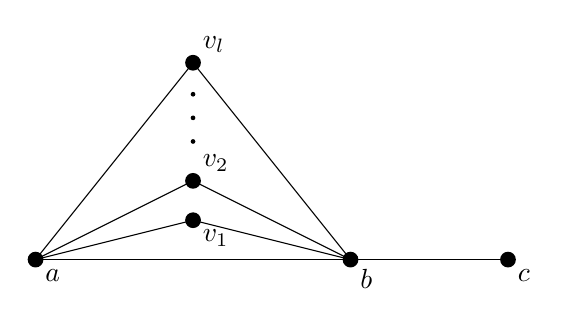
\begin{tikzpicture}
\draw (0,1) -- (4,1);
\draw (4,1) -- (6,1);
\draw (0,1) -- (2,1.5);
\draw (4,1) -- (2,1.5);
\draw (0,1) -- (2,2);
\draw (4,1) -- (2,2);
\draw (0,1) -- (2,3.5);
\draw (4,1) -- (2,3.5);

\fill (0,1) circle(0.1cm) node[anchor=north west] {$a$};
\fill (4,1) circle(0.1cm) node[anchor=north west] {$b$};
\fill (6,1) circle(0.1cm) node[anchor=north west] {$c$};
\fill (2,1.5) circle(0.1cm) node[anchor=north west] {$v_1$};
\fill (2,2) circle(0.1cm) node[anchor=south west] {$v_2$};
\fill (2,3.5) circle(0.1cm) node[anchor=south west] {$v_l$};
\fill (2,2.5) circle(0.3mm);
\fill (2,2.8) circle(0.3mm);
\fill (2,3.1) circle(0.3mm);

\end{tikzpicture}
\caption{Graph $G$}
\end{figure}
\end{proof}

\begin{proposition}
The following results hold:
\end{proposition}
\noindent (i.) For $n \geq 3$, let $T$ be a tree,  $\gamma_{spc}(T)=n$\\
(ii.) For $n \geq 4$, let $C_n$ be a cycle,  $\gamma_{spc}(C_n)=n$\\
(iii.) For $r,s \geq 2$, let $K_{r,s}$ be a complete bipartite graph,   $\gamma_{spc}(K_{r,s})=r+s$\\
(iv.) For $p,q \geq 2$, let $Wd_{p,q}$ be a windmill graph,  $\gamma_{spc}(Wd_{p,q})=q+1$.
\begin{proof}
(i.) In a tree $T$, either a vertex is a cut-vertex or a pendant vertex. Hence by proposition 4.2.1, $\gamma_{spc}(T)=n$.\\
(ii.) By contradiction, assume  $\gamma_{spc}(C_n) < n$. Let $S$ be a SPCDS of $C_n$, with $|S| < n$. And let $u$ be a vertex of $C_n$ and $v,w$ be its neighbors. If $u \notin S$, then to dominate $u$ either $v$ or $w$ or both must be in $S$. Now consider the following cases:\\
\textit{Case }1: $v,w \in S$. Clearly $|S| \leq n-1$. But vertex $u$ is defended by $v~ \&~ w$, which is a contradiction.\\
\textit{Case }2: $v\in S$ and $w \notin S$. Clearly $|S| \leq n-2$. But $(S\setminus \lbrace v \rbrace) \cup \lbrace u \rbrace$ becomes disconnected, which is a contradiction.\\
\textit{Case }3: $v \notin S$ and $w \in S$. Same as case 2.\\
Hence $\gamma_{spc}(C_n) = n$.\\
(iii.) Let $X = \lbrace x_1,x_2,...,x_r\rbrace $ and $Y=\lbrace y_1,y_2,...,y_s \rbrace $ be the bipartition of $K_{r,s}$. By contradiction, assume $\gamma_{spc}(K_{r,s}) < r+s$. Let $S$ be a SPCDS of $K_{r,s}$ with $|S| < r+s$. Then consider the following cases:\\
\textit{Case }1: $|S \cap X| < |X|$. In this case, some vertex $x$ exists in $G$ such that $x \in X$, $x \notin S$ and is defended by all the vertices of $S \cap Y$, which is a contradiction.\\
\textit{Case }2: $|S \cap Y| < |Y|$. Same as case 1.\\
Hence $\gamma_{spc}(K_{r,s}) = r+s$.\\
(iv.) Let $G \cong Wd_{p,q}$ and $v_c$ be the common center vertex. Since $v_c$ is a cut-vertex, by proposition 4.2.1, $v_c$ is part of every SPCDS of $G$. Clearly, $\gamma_{spc}(G) \geq q+1$, as there are $q$ connected components in $G \setminus \lbrace v_c \rbrace$. It can be easily to verify that a vertex from each connected component of $G \setminus \{ v_c \}$ and a set which contains $v_c$ is a SPCDS of $G$. Hence $\gamma_{spc}(G) \leq q+1$. Therefore $\gamma_{spc}(Wd_{p,q})=q+1$.
\end{proof}
\noindent The following corollary follows from statement (i) of Proposition 4.2.1.
\newtheorem{Corly}{Corollary}
\begin{Corly}
Let $P$ be a path with $n \geq 3$, then $\gamma_{spc}(p)=n$.
\end{Corly}

\begin{proposition}
Let $k,n$ be two non-negative integers and $W_n$ be a wheel graph with $n \geq 7$ vertices, then
\[
\gamma_{spc}(W_n) = \begin{cases}
k+1, & \text{for }n=3k+1 \\
k+2, & \text{for }n=3k+2 \\
k+3, & \text{for }n=3k+3. \\
\end{cases} 
\]
\end{proposition}
\begin{proof}
The vertices of $W_n$ are labeled as $V(W_n)= \{ v_1, v_2,...,v_n\}$ such that $v_1, v_2,...,v_{n-1}$ is a cycle of length $n-1$. Let
\[
S = \begin{cases}
\lbrace v_{3i+1}:0\leq i < k \rbrace \cup \lbrace v_{3k+1} \rbrace, & \text{if }n=3k+1 \\
\lbrace v_{3i+1}:0\leq i < k \rbrace \cup \lbrace v_{3k+1},v_{3k+2} \rbrace, & \text{if }n=3k+2 \\
\lbrace v_{3i+1}:0\leq i < k \rbrace \cup \lbrace v_{3k+1},v_{3k+2},v_{3k+3} \rbrace, & \text{if }n=3k+3. \\
\end{cases} 
\]
Clearly $S$ is a CDS of $W_n$. For every vertex $u \in S \setminus V(W_n)$, there exists a unique vertex $v \in S$ such that $(S \setminus \lbrace v \rbrace) \cup \lbrace u \rbrace$ is a CDS of $W_n$. Hence $S$ is a SPCDS of $W_n$ and $\gamma_{spc}(W_n) \leq |S|$.\\
The following claim is useful in proving the lower bound.\\
\textbf{Claim} : $v_n$ is part of every SPCDS of $W_n$.\\
\textit{Proof of claim} : By contradiction, assume $S$ be a SPCDS of $W_n$ and $v_n \notin S$. Since $n \geq 7$, $|S \cap \lbrace v_1, v_2, ... , v_{n-1} \rbrace | \geq 2$ and so there exists at least two vertices by which $v_n$ is defended, which contradicts our assumption that $S$ is a SPCDS of $W_n$. Hence $v_n \in S$. \\
Next we show that $\gamma_{spc}(W_n) \geq k+3$ if $n \geq 7 $ and $n=3k+3$. \\
By contradiction, assume that $\gamma_{spc}(W_n) < k+3$. Since $v_n$ is part of every SPCDS of $W_n$, $| \lbrace v_1,v_2,...,v_{n-1} \rbrace \cap S | < k+2$. Now, there exists two vertices $v_i,v_j \in S \cap \lbrace v_1,v_2,..., v_{n-1} \rbrace $, such that $( v_{i+1},...,v_{j-1}) \cap S = \phi$ and $j-i > 3$ or $j-i=2$. If $j-i=2$, then vertex $v_{i+1}$ is defended by two of its neighbors, which is a contradiction. If $j-i > 3$, then $ v_{i+2}$ is dominated by only $v_n$ but $(S\setminus \lbrace v_n \rbrace) \cup \lbrace v_{i+2} \rbrace$ is not connected, a contradiction. Hence $\gamma_{spc}(W_n) \geq k+3$. Therefore $\gamma_{spc}(W_n) = k+3$, if $n=3k+3$. Similarly we can prove for $n=3k+1$ and $n=3k+2$.
\end{proof}

\begin{proposition}
Let $k,n$ be two non-negative integers and $F_n$ be the fan graph with $n \geq 5$ vertices, then 
\[
\gamma_{spc}(F_n) = \begin{cases}
k+2, & \text{for }n=3k+2 \\
k+3, & \text{for }n=3k+3 \\
k+4, & \text{for }n=3k+4. \\
\end{cases} 
\]
\end{proposition}
\begin{proof}
The vertices of $F_n$ are labeled as $V(F_n)= \{ v_1, v_2,...,v_n\}$ such that $v_1, v_2,...,v_{n-1}$ is a path of length $n-1$.  Let
\[
S = \begin{cases}
\lbrace v_{3i+1}:0\leq i < k \rbrace \cup \lbrace v_{3k+1},v_{3k+2} \rbrace, & \text{if }n=3k+2 \\
\lbrace v_{3i+1}:0\leq i < k \rbrace \cup \lbrace v_{3k+1},v_{3k+2},v_{3k+3} \rbrace, & \text{if }n=3k+3 \\
\lbrace v_{3i+1}:0\leq i < k \rbrace \cup \lbrace v_{3k+1},v_{3k+2},v_{3k+3},v_{3k+4} \rbrace, & \text{if }n=3k+4. \\
\end{cases} 
\]
Clearly $S$ is a SPCDS of $F_n$ and $\gamma_{spc}(F_n) \leq |S|$. With similar argument given in proposition 4.2.7, we can prove that $\gamma_{spc}(F_n) \geq |S|$. Hence the result.
\end{proof}
\chapter{Algorithmic Complexity of Variants of Perfect Connected Domination in Graphs} 
\noindent
This chapter presents the NP-completeness result obtained for the decision version of perfect connected domination and secure perfect connected domination problem.
\section{Complexity of Perfect Connected Domination}
\noindent
This section contains algorithmic complexity result obtained for bipartite graphs for the problem of perfect connected domination problem.
\subsection{Perfect connected domination in bipartite graphs}
\noindent  
Decision version of the perfect connected domination problem for bipartite graphs is defined as follows:\\
\textbf{PERFECT CONNECTED DOMINATION BIPARTITE GRAPHS (PCDOMB)}\\
\indent \textbf{Instance:} A connected bipartite graph $G=(V,E)$ and a positive integer $l$.\\
\indent \textbf{Question:} Does there exist a PCDS of size at most $l$ in $G$?\\
For proving PCDOMB is NP-complete, we reduce from a NP-complete problem EXACT 3 SET COVER, as defined below:\\
\textbf{EXACT 3 SET COVER (X3C)}\\
\indent \textbf{Instance:} A finite set $X$, $|X|=3q$ for an integer $q$ and a collection $C$ of 3-element subsets of $X$.\\
\indent \textbf{Question:} Does there exist a $C' \subseteq C$ such that every element of $X$ occurs exactly in one \\ 
\indent \indent \indent \indent   \hspace{1ex} member of $C'$?

%\newtheorem{theorem}{Theorem}
\begin{theorem}
PCDOMB is NP-complete.
\begin{proof}
Clearly, the PCDS can be checked in polynomial time hence PCDOMB is a member of NP.\\
Assume that we have an arbitrary instance of X3C as $X=\lbrace x_1,\ldots ,x_{3q} \rbrace$ and $C=\lbrace c_1, \ldots,c_m \rbrace$. We construct a bipartite graph $G=(V,E)$ from the instance eof X3C as follows. Each element of $X$ add a new vertex in $G$ and each element of $C$ add a path $P_2:u_i-c_i$ in $G$. There is an edge between vertices of $X$ and $C$ if $x_i \in c_j$. Along with these vertices two $P_2$ namely $p_1-p_2, r_1-r_2$ are added and $p_1$ is made adjacent to each vertex $c_i$ where $1 \leq i \leq m$ and $r_1$ is made adjacent to each vertex $u_i$ where $1 \leq i \leq m$. Thus $V = A \cup B$, where $A=\lbrace c_i : 1 \leq i \leq m \rbrace \cup \lbrace p_2, r_1 \rbrace $ and $B=\lbrace x_i : 1 \leq i \leq 3q \rbrace \cup \lbrace u_i : 1 \leq i \leq m \rbrace \cup \lbrace p_1, r_2 \rbrace $; $E=\lbrace (c_i,u_i): 1\leq i \leq m \rbrace \cup \lbrace (c_i,x_j):1 \leq i \leq m$ $,$ $1 \leq j \leq 3q$ $\&$ $ x_j \in c_i \rbrace \cup \lbrace (p_1,c_i), (r_1,u_i): 1\leq i \leq m \rbrace \cup \lbrace (p_1,p_2),(r_1,r_2) \rbrace $. Clearly the constructed graph $G$ with $|V|=2m+3q+4$ and  $|E|=6m+2$ is a bipartite graph. Thus in polynomial time, from an instance of X3C we can construct graph $G$. Further we show that X3C has a solution if and only if a PCDS of at most $k=2q+2$ size in $G$.\\
Let $C'$ be a solution of X3C and let $D = \lbrace c_i,u_i : c_i \in C' \rbrace \cup \lbrace p_1,r_1 \rbrace$. Clearly $|D|=2q+2$. All the vertices of $X$ are dominated by unique vertex of $C$ and $\forall c_i, c_i \notin D$ and $p_2$ are dominated by unique vertex $p_1$ and similarly, $\forall u_i, u_i \notin D$ and $r_2$ are dominated by unique vertex $r_1$. Vertices's $p_1,r_1$ is connected to each $c_i,u_i$ respectively and $c_i,u_i$ is $P_2$, $G[D]$ is connected. Hence $D$ is a PCDS of $G$.\\ 
Conversely, assume that a PCDS $D$ of $G$ of size at most $2q+2$. Then the following claims hold:\\
{\textit{Claim 1}:} $p_1,r_1 \in D$.\\
\textit{Proof of claim.} By contradiction, if $p_1 \notin D$ (or $r_1 \notin D$), then if $p_2 \in D$ $(r_2 \in D)$ then $G[D]$ is not connected otherwise $p_2$ $(r_2)$ is undominated, which is a contradiction.\\
{\textit{Claim 2}:} If $c_i \in D$ then $u_i \in D$ and vice-versa.\\
\textit{Proof of claim.} By contradiction, assume $\exists c_a, c_a\in D$ and $u_a \notin D$. Clearly $u_a$ is dominated by both $c_a$ and $r_1$, which is a contradiction i.e. $D$ is not a PCDS of $G$. Similarly, the converse can be proved.\\
{\textit{Claim 3}:} $\forall x_i, x_i \notin D$.\\
\textit{Proof of claim.} By contradiction, let there be a vertex $x_a \in D$. Since $G[D]$ is connected, there exists a vertex $c_b \in D$ where $c_b \in N(x_a)$ and from claim 1 and claim 2 it follows that, $u_b \in D$. Let $D' = D\setminus \lbrace p_1,r_1,x_a,c_b,u_b \rbrace$. Clearly $|D'| \leq 2q-3$. To dominate $(X\setminus x_a)$, from claim 2, set $D'$ must contain at least $2q-2$ vertices, which contradicts with our assumption that $|D| \leq 2q+2$.\\
Thus, it follows that for all $x_i$, $x_i \notin D$.\\
Let $C'=\lbrace c_i : c_i \in D \rbrace$. From claim 3, a unique $c_j$ dominates each vertex $x_i \in X$, thus $C'$ is a solution of X3C.\\
Hence PCDOMB is NP-complete.
\end{proof}
\end{theorem}
\section{Complexity of Secure Perfect Connected Domination}
\noindent
This section contains the result obtained for finding a minimum SPCDS of $G$ of at most $k$ size is proved NP-complete. Further we also show that for bipartite graphs and star convex bipartite graphs the problem is still NP-complete.
\subsection{Secure perfect connected domination in arbitrary graphs}
\noindent
\noindent Decision version of the secure perfect connected domination problem is defined as follows:\\
\textbf{SECURE PERFECT CONNECTED DOMINATION (SPCDOM)}\\
\indent \textbf{Instance :} A simple, undirected, connected graph $G=(V,E)$ and a positive integer $k$.\\
\indent \textbf{Question :} Is $\gamma_{spc}(G) \leq k$?\\
For proving the NP-completeness of the SPCDOM, we reduce from the following know NP-complete problem \cite{Yen}.\\
\textbf{PERFECT DOMINATION (PDOM)}\\
\indent \textbf{Instance :} A simple, undirected, connected graph $G=(V,E)$ and a positive integer $l$.\\
\indent \textbf{Question :} Does there exist a PDS of size at most $l$ in $G$?
%\newtheorem{theorem}{Theorem}
\begin{theorem}
SPCDOM is NP-complete.
\end{theorem}
\begin{proof}
First we show that SPCDOM is a member of NP. For a set $S \subseteq V(G)$, each vertex in $V(G) \setminus S$, we can check in polynomial time that a unique vertex in $S$ exists which defends that vertex. Next we show how to reduce an instance of PDOM to an instance of SPCDOM.\smallskip \\ 
We construct a graph $G^*=(V,E)$ as an instance of SPCDOM from the instance of PCDOM as follows. We add two new vertices and $|V(G)|+1$ new edges in $G^*$ such that $V(G^*)=V(G) \cup \lbrace x,y \rbrace$ and  $E(G^*)=E(G) \cup \lbrace (x,v):x \neq v ~\&~v \in V(G^*) \rbrace$. Hence, the graph $G^*$ can be constructed easily in polynomial time from $G$. Further we show that a PDS of at most $k$ size in $G$ if and only if a SPCDS of at most $k+2$ size in $G^*$.\\
Let $|D| \leq k$ be a PDS of $G$ and $S=D \cup \lbrace x,y \rbrace$. Clearly $|S| \leq k+2$, $G^*[S]$ is connected and each vertex in $ V(G^*) \setminus S$ is dominated by exactly one vertex in $\{x,y\}$ and exactly one vertex in $S \setminus \{x,y\}$. Also no vertex in $V(G^*) \setminus S$ can be defended by vertices in $\{x,y\}$. Hence a unique vertex in $S$ defends each vertex in $ V(G^*)\setminus S$ in $G^*$. Thus $S$ is a SPCDS of $G^*$.\\
Conversely, assume $S$ be a SPCDS of $G^*$ with $|S| \leq k+2$. Since $x$ is a cut-vertex and $y$ is a pendant vertex in $G^*$, by proposition 4.2.1, $x,y \in S$. Since $x$ can not defend any vertex in $G^*$, $\forall u \in V(G^*)\setminus S$, a unique vertex $v \in S\setminus \lbrace x,y \rbrace $ must exist such that $(S \setminus \lbrace v \rbrace) \cup \lbrace u \rbrace$ is a CDS of $G^*$ i.e. $v$ is uniquely dominated by $u$. Hence $D = S \setminus \lbrace x,y \rbrace$ is a PDS of $G$ and clearly, $|D| \leq k$.\\
Hence SPCDOM is NP-complete.
\end{proof}
\subsection{Secure perfect connected domination in bipartite graphs}
\noindent  
For bipartite graphs, decision version of the secure perfect connected domination problem is defined as follows:\\
\textbf{SECURE PERFECT CONNECTED DOMINATION BIPARTITE GRAPHS (SPCDOMB)}\\
\indent \textbf{Instance:} \hspace{1ex}A connected bipartite graph $G=(V,E)$ and a positive integer $k$.\\
\indent \textbf{Question:} Is $\gamma_{spc}(G) \leq k$?\\
For proving SPCDOMB is NP-complete, we reduce from EXACT 3 SET COVER.

\begin{theorem}
SPCDOMB is NP-complete.
\begin{proof}
Clearly, SPCDOMB is a member of NP.\\
\noindent Assume that we have an arbitrary instance of X3C as $X=\lbrace x_1,\ldots ,x_{3q} \rbrace$ and $C=\lbrace c_1, \ldots,c_m \rbrace$. We construct a bipartite graph $G=(V,E)$ from the given instance of X3C as follows. Each element of $X$ create a new vertex in $G$ and each element of $C$ create a path $P_2:u_i-c_i$ in $G$. There is an edge between vertices of $X$ and $C$ if $x_i \in c_j$. Along with these vertices two path $P_2$ namely $p_1-p_2, r_1-r_2$ are added and $p_1$ is made adjacent to each vertex $c_i$ where $1 \leq i \leq m$ and $r_1$ is made adjacent to each vertex $u_i$ where $1 \leq i \leq m$ and $x_j$ where $1 \leq j \leq 3q$. Thus $V = A \cup B$, where $A=\lbrace c_i : 1 \leq i \leq m \rbrace \cup \lbrace p_2, r_1 \rbrace $ and $B=\lbrace x_i : 1 \leq i \leq 3q \rbrace \cup \lbrace u_i : 1 \leq i \leq m \rbrace \cup \lbrace p_1, r_2 \rbrace $; $E=\lbrace (c_i,u_i): 1\leq i \leq m \rbrace \cup \lbrace (c_i,x_j):1 \leq i \leq m$ $,$ $1 \leq j \leq 3q$ $\&$ $ x_j \in c_i \rbrace \cup \lbrace (p_1,c_i), (r_1,u_i): 1\leq i \leq m \rbrace \cup \lbrace (r_1,x_i): 1\leq i \leq 3q \rbrace \cup \lbrace (p_1,p_2),(r_1,r_2),(p_1,r_1) \rbrace $. Clearly the constructed graph $G$ with $|V|=2m+3q+4$ and  $|E|=6m+3q+3$ is a bipartite graph. Thus in polynomial time from an instance of X3C we can construct graph $G$. Further we shall show that X3C has a solution if and only if a SPCDS of at most $k=m+4$ size in $G$.\\
Let $C'$ be a solution of X3C and let $S = \lbrace c_i:c_i \in C' \rbrace \cup \lbrace u_i:c_i \notin C' \rbrace \cup \lbrace p_1,p_2,r_1,r_2 \rbrace$. Clearly $|S|=m+4$. Each vertex $x_i$, there exist a unique vertex $c_j \in S $ where $(x_i,c_j)\in E$ such that $(S\setminus \lbrace c_j \rbrace) \cup \lbrace x_i \rbrace $ is a CDS of $G$. And each vertex $c_i,u_i\in (V \setminus S)$, a corresponding vertex $u_i,c_i \in S$ exists such that $(S\setminus \lbrace u_i \rbrace) \cup \lbrace c_i \rbrace$ and $(S\setminus \lbrace c_i \rbrace) \cup \lbrace u_i \rbrace $ respectively is a CDS of $G$. Since neighbor of each vertex of $c_i$ contains $p_1$ and neighbor of each vertex of $u_i$ contains $r_1$ and $p_1,r_1$ is also adjacent to each other, $G[S]$ is connected. Hence set $S$ is a SPCDS of $G$.\\
Conversely, assume that a SPCDS $S$ of size at most $m+4$ in $G$. From proposition 4.2.1, it is clear that $ \lbrace p_1,p_2,r_1,r_2 \rbrace \in S$. Then the following claims hold:\\
{\textit{Claim 1}:} If $c_i \in S$ then $u_i \notin S$ and vice-versa.\\
\textit{Proof of claim.} Consider the following cases:\\
\textbf{Case 1:} By contradiction, assume $\exists c_a, c_a\in S$ and $u_a \in S$. Let $S'=S \setminus \lbrace p_1,p_2,r_1,r_2,c_a,u_a \rbrace$ and $|S'| \leq m-2$. Irrespective of $x_i \in S$, there exist at least one pair $(u_j,c_j) \notin S$ such that $(S \setminus \lbrace r_1 \rbrace ) \cup \lbrace u_j \rbrace $, vertex $r_2$ becomes disconnected which is a contradiction.\\ 
\textbf{Case 2:} By contradiction, assume $\exists u_a, u_a\in S$ and $c_a \in S$. Let $S'=S \setminus \lbrace p_1,p_2,r_1,r_2,c_a,u_a \rbrace$ and $|S'| \leq m-2$. Similar to case 1, irrespective of $x_i \in S$, there exist at least one pair $(u_j,c_j) \notin S$ such that $(S \setminus \lbrace r_1 \rbrace ) \cup \lbrace u_j \rbrace $, vertex $r_2$ becomes disconnected which is a contradiction.\\ 
From above case 1,2, it follows that claim holds i.e. if $u_i\in S$ then $c_i \notin S$ and vice-versa.\\
{\textit{Claim 2}:} $\forall x_i, x_i \notin S$.\\
\textit{Proof of claim.} By contradiction, assume there exist a vertex $x_a \in S$. Let $S' = S \setminus \lbrace p_1,p_2,r_1,r_2,x_a \rbrace$ and $|S'| \leq m-1$. From claim 1, either $u_j$ or $c_j$ is in $S$. Then there exist at least one pair $(u_k,c_k) \notin S$ such that $(S \setminus \lbrace r_1 \rbrace ) \cup \lbrace u_k \rbrace $, vertex $r_2$ becomes disconnected which is a contradiction.\\ 
Thus, it follows that the claim holds i.e. for all $x_i$, $x_i \notin S$.\\
Let $C'=\lbrace c_i : c_i \in S \rbrace$. From claim 2 and 3, each $x_i \in X$ is defended by unique $c_j \in S$, thus $C'$ is a solution of X3C.\\
Hence SPCDOMB is NP-complete.
\end{proof}
\end{theorem}
\subsection{Secure perfect connected domination in star convex bipartite graphs}
\noindent 
Decision version of the secure perfect connected domination problem for star convex bipartite graphs is defined as follows:\\
\textbf{SECURE PERFECT CONNECTED DOMINATION STAR CONVEX BIPARTITE GRAPHS (SPCDSCB)}\\
\indent \textbf{Instance:} A simple, undirected, connected graph $G=(V,E)$ and a positive integer $k$.\\
\indent \textbf{Question:} Is $\gamma_{spc}(G) \leq k$?\\
For proving the NP-completeness of the SPCDOM, we reduce from the know NP-complete perfect domination problem \cite{Yen}.
\begin{theorem}
SPCDSCB is NP-complete.
\begin{proof}
Given a subset of vertices is a SPCDS can be verified in polynomial time, hence SPCDSCB is a member of NP.\\
Given an arbitrary instance of bipartite graph $G=(X,Y,E)$ and positive integer $k$, we construct star convex bipartite graph $G^*=(X^*, Y^*, E^*)$ as follows. Add two path $P_2$ namely $x-x_0$ and $y-y_0$ in graph $G$ and made vertex $x$ adjacent to every vertex belongs to $Y$ and vertex $y$ is made adjacent to every vertex belongs to $X$. Thus $X^*=X \cup \lbrace x_0,x \rbrace$ and $Y^*=Y \cup \lbrace y_0,y \rbrace$; $E^*=E \cup \lbrace (x,v): v \in X \rbrace \cup \lbrace (y,v): v \in Y \rbrace \cup \lbrace (x,y),(x_0,y), (x,y_0) \rbrace$. Clearly the constructed graph $G^*$ is a star convex bipartite graph with star defined on $T=(X,F)$ where $F=((x,v):v \in (X \cup \lbrace x_0 \rbrace)$ as the neighbor of each vertex in $Y$ contains vertex $x$. Further we show that graph a PDS of at most $k$ size in $G$ if and only if a SPCDS of at most $k+4$ size in graph $G^*$.\smallskip \\
Assume $|D| \leq k$ be a PDS of $G$. Let $S=D \cup \lbrace x_0,x,y_0,y \rbrace$. Clearly $|S| \leq k+4$ and $G^*[S]$ is connected. Since a unique vertex $u \in D$ dominates each vertex in $v \in (V \setminus D)$. Hence each vertex $v \in (V^*\setminus S)$ are defended by a unique vertex $u \in S$. Thus set $S$ of at most $k+4$ size is a SPCDS of $G^*$.\smallskip \\
Conversely, assume $S$ be a SPCDS of $G^*$ with $|S| \leq k+4$. By proposition 4.2.1, $x_0,x,y_0,y \in S$. Since $x_0$ and $y_0$ can not defends any vertex in $G^*$. Hence $\forall u \in (V^*\setminus S)$, a unique vertex $v \in (S\setminus \lbrace x_0,x,y_0,y \rbrace) $ must exists such that the set $(S \setminus \lbrace v \rbrace) \cup \lbrace u \rbrace$ of $G^*$ is a CDS i.e. $u$ is uniquely dominated by $v$. Hence $D = S \setminus \lbrace x_0,x,y_0,y \rbrace$ is a PDS of $G$ and clearly, $|D| \leq k$.\\
Hence SPCDSCB is NP-complete.
\end{proof}
\end{theorem}
\chapter{Parameterized Complexity of Variants of Connected Domination in Graphs} 
\noindent
In this chapter, we presents the result obtained for parameterized complexity of the decision version of doubly connected domination and secure doubly connected domination problem.
\section{Parameterized Complexity of Doubly Connected Domination}
\noindent
This section contains parameterized complexity result of a doubly connected domination problem for bipartite and split graphs.
\subsection{Doubly connected domination in bipartite graphs}
\noindent 
For bipartite graphs, the parameterized version of the doubly connected domination problem is defined as follows:\\
\textbf{DOUBLY CONNECTED DOMINATION BIPARTITE GRAPHS (DCDB)}\\
\indent \textbf{Instance :} A connected bipartite graph $G$ and a positive integer $k$.\\
\indent \textbf{Parameter :} $k$.\\
\indent \textbf{Question :} Does $G$ have a DCDS of size at most $k$? \smallskip

\noindent For proving DCDB is W[2]-hard, we reduce from W[2]-hard problem DOMINATION \cite{ppc}, defined as follows:\\
\textbf{DOMINATION (DOM)}\\
\indent \textbf{Instance :} A simple, undirected and connected graph $G=(V,E)$ and a positive integer $k$.\\
\indent \textbf{Parameter :} $k$.\\
\indent \textbf{Question :} Does $G$ have a DS of size at most $k$?
\begin{theorem}
DCDB is W[2]-hard.
\end{theorem}
\begin{proof}
From the NP-hardness proof of doubly connected domination in bipartite graphs \cite{dcds} and the fact that DOM is W[2]-hard, it follows that DCDB is W[2]-hard.
\end{proof}
%%%%%%%%%%%%%%%%%%%%%%%%%%%%%%%%
%%%%%%%%%%%%%%%%%%%%%%%%%%%%%%%%%
\subsection{Doubly connected domination in split graphs}
\noindent 
For split graphs, the parameterized version of the doubly connected domination problem is defined as follows:\\
\textbf{DOUBLY CONNECTED DOMINATION SPLIT GRAPHS (DCDMS)}\\
\indent \textbf{Instance :} A connected split graph $G$ and a positive integer $k$.\\
\indent \textbf{Parameter :} $k$.\\
\indent \textbf{Question :} Does there exist a DCDS of size at most $k$?\\
For proving DCDMS is W[2]-hard, we reduce from known W[2]-hard DOM problem.
\begin{theorem}
DCDMS is W[2]-hard.
\end{theorem}
\begin{proof}
Given a positive integer $k$ and an instance of $G=(V,E)$ of DS, we construct a split graph $G^*=(V,E)$ whose the vertex set $V(G^*)$ is partitioned into two disjoint subsets a maximum clique $Q$ and an independent set $I$. We create two vertices in $G^*$ for each vertex $x \in V(G)$ such that one belongs to $Q$ and other $I$. Thus $|Q|=|I|$. If there is an edge between $u$ and $v$ in $G$ then add edge between $u$ and $v$ in $G^*$, $u \in Q$, $v \in I$ and add edge between $v$ and $u$ in $G^*$, $v \in Q$, $u \in I$. Thus $V(G^*)=Q \cup I$ and $E(G^*)=\lbrace (x_i,x_j): 1 \leq i,j \leq n ~\&~ i \neq j~\&~ (x_i, x_j) \in E(G)~\&~ x_i \in Q~\&~ x_j \in I \rbrace \cup \lbrace (x_i,x_i): 1 \leq i \leq n~\&~ x_i \in Q~\&~ x_i \in I \rbrace \cup \lbrace (x_i,x_j): 1 \leq i,j \leq n~\&~ i \neq j~\&~ (x_i,x_j) \in Q \rbrace  $. Clearly, in polynomial time, the constructed graph $G^*$  from $G$ is a split graph. Further we show that a DS of at most $k$ size in $G$ if and only if a DCDS of at most $k$ size in $G^*$.\\
Assume $|D| \leq k$ be a DS of $G$. Let $D' = \lbrace x_i: x_i \in D~\&~ x_i \in Q \rbrace $, thus $|D'| \leq k$. Each vertex in $D'$ belongs to $Q$, $G^*[D']$ is connected and vertices in $(V(G^*)\setminus D') \cap Q$ are dominated. Since vertices of $D$ dominates every vertex in $V(G)\setminus D$, hence every vertex of $(V(G^*)\setminus D') \cap I$ is also dominated by at least one vertex of $D'$. Since every vertex of $I$ is dominated and also $Q$ and $I$ are mirrors of each other. Hence $G^*[V(G^*) \setminus D']$ is connected. Thus $D'$ is a DCDS of $G^*$.\\
Assume that $|D'|$ be a DCDS of $G^*$. Consider the following cases:\\
\textit{Case 1:} If $D' \cap Q \neq \phi$ and $D' \cap I = \phi$. Clearly, each vertex $u \in I$ gets dominated by at least one vertex in $D'$. Hence each vertex in $V(G) \setminus D'$ is dominated by $D'$. Thus $D'$ is a DS of $G$ with $|D'| \leq k$.\\
\textit{Case 2:} $D' \cap Q \neq \phi$ and $D' \cap I \neq \phi$. Replace each vertex $u \in D' \cap I$ with the corresponding vertex (i.e. mirror vertex) $u' \in Q$ to obtain $D''$. The modified set $D''$ contains only vertices from $Q$, $|Q| \leq k$ and is a DCDS of $G^*$. It follows from the similar argument given in case 1 that $D''$ is a DS of $G$.\\
Thus DCDMS is W[2]-hard.
\end{proof}

%%%%%%%%%%%%%%%%%%%%%%%%%%%%%
\section{Parameterized Complexity of Secure Doubly Connected Domination}
%%%%%%%%%%%%%%%%%%%%%%%%%%%%%
\noindent
This section contains parameterized complexity result of a secure doubly connected domination problem for split graphs. 
\subsection{Secure doubly connected domination in split graphs}
\noindent For split graphs, the parameterized version of the secure doubly connected domination problem is defined as follows:\\ 
 \textbf{SECURE DOUBLY CONNECTED DOMINATION SPLIT GRAPHS (SDCD)}\\
\indent \textbf{Instance :} A connected split graph $G=(V,E)$ and a positive integer $k$.\\
\indent \textbf{Parameter :} $k$.\\
\indent \textbf{Question :} Does there exists a SDCDS of size at most $k$?\\
For proving SDCD is W[2]-hard, we reduce from DCDMS which has been proved as W[2]-hard in Theorem 6.1.2.

\begin{theorem}
SDCD is W[2]-hard.
\end{theorem}
\begin{proof}
Given a positive integer $k$ and a split graph $G=(V,E)$ whose vertex set is partitioned into two disjoint subsets, a maximum clique $Q$ and an independent set $I$. We construct another split graph $G^*=(V,E)$ from $G$ such that the vertex set is partitioned into two subsets a clique $Q^*$ and an independent set $I^*$. $V(G^*) = V(G) \cup \lbrace x \rbrace $, where $x$ is a additional vertex. $E(G^*) = E(G) \cup \lbrace (x, u) : \forall u \in Q\rbrace \cup \lbrace (x, v) : \forall v \in I$ $\&$ $d_G(v) > 1\rbrace $. The graph $G^*$ is constructed in polynomial time is a split graph, where the clique vertex set $Q^*=Q\cup \lbrace x \rbrace$ and independent vertex set $I^*=I$. Also $|V(G^*)| = |V(G)|+1$ and $|E(G^*)|=|E(G)|+|V(G)|-n_1(G)$, where $n_1(G)$ denotes number of pendant vertices. Further we show that a DCDS of at most $k$ size in $G$ if and only if a SDCDS of at most $k + 1$ size  in $G^*$. \\
\noindent Assume that $|D| \leq k$ be a DCDS of graph $G$. Let $S=D \cup \lbrace x \rbrace$ with $|S|\leq k+1$. The set S is a SDS as $\forall v \in V(G^*)\setminus S$, $(S\setminus \lbrace x \rbrace) \cup \lbrace v \rbrace$ in $G^*$ is a DCDS. The graphs $G^*[V(G^*)\setminus S]$ and $G^*[S]$ are also connected, hence set S is a SDCDS of $G^*$.\\
Conversely, suppose $|S| \leq k+1$ is a SDCDS of graph $G^*$. We have two cases:\\
\textit{Case 1:} $x \in S$. Let $S'=S \cap V(G)$. Clearly $|S'| \leq k$. Consider the following two sub cases:\\
\textit{Case 1.1:} $G[ S']$ \textit{is connected}. Clearly the graph $G[V(G) \setminus S']$ is connected. To prove that the set $S'$ is a DS of $G$, by contradiction, assume that $S'$ is not a DS of $G$. A vertex $v \in V(G)\setminus S'$ exists in $G$ such that $N[v] \cap S' = \phi$. Which implies that vertex $v$ was only dominated by $x$ in $G^*$ and the graph $G^*[ (S \setminus \lbrace x \rbrace) \cup \lbrace v \rbrace]$ is not connected, which is a contradiction. Hence $S'$ is a DS of $G$. Therefore $S'$ is a DCDS of $G$.\\
\textit{Case 1.2:} $G[ S']$ \textit{is not connected}. Since graph $G$ is a split graph, hence there exists at least one isolated vertex $w \in (S' \cap I)$ in $G[S']$. Let $W = \lbrace w:d_{G[ S']}(w) = 0 \hspace{1ex} \& \hspace{1ex} w \in S' \rbrace $. Since $G^*[ S ]$ is connected, all the vertices in $W$ are only adjacent to $x$ in $G^*[ S]$. From the construction of graph $G^*$, clearly $d_G(w) > 1 $, $\forall w \in W$. Replace an isolated vertex $w$ in $G[ S']$ with a vertex in $N_G[w]$ in $G[ V(G) \setminus S' ]$ until $G[S']$ becomes connected. Let $S''$ be the modified $S'$ set. Clearly $|S''| = |S'|$ and $G[ V(G)\setminus S'']$ is also connected as $d_G(w) > 1$. From Case 1.1 it follows that, $S''$ is also a DS of $G$. Hence $S''$ is a DCDS of $G$.\\
\textit{Case 2:} $x \notin S$. Let $R= (S\setminus \lbrace v \rbrace) \cup \lbrace x \rbrace $, where $v \in S$. By definition of SDCDS, $R$ is a DCDS of $G^*$. From the construction of $G^*$, it follows that $N(v) \subseteq N(x)$. Therefore $R$ is a SDCDS of $G^*$.\\
Since $x \in R$, by applying Case 1 we can get a DCDS of $G$ of size at most $k$ from $R$. Hence SDCD is W[2]-hard.
\end{proof}


\chapter{Conclusion and Future Research} 
\noindent
In this thesis we studied the algorithmic complexity of three variant of connected domination, namely, doubly connected domination, secure doubly connected domination and secure perfect connected domination for some classes of graphs. In chapter 3, we proved that for split graphs, chordal bipartite graphs and star convex bipartite graphs the DCDOM is NP-complete. And in chapter 6, for split graphs and bipartite graphs, we proved that DCDOM is still W[2]-hard. In chapter 3, for split graphs and chordal bipartite graphs, we proved that SDCDOM is NP-complete. And in chapter 6, we proved that SDCDOM is still W[2]-hard for split graphs. In chapter 5, We proved that PCDOM is NP-complete even when restricted to bipartite graphs. In chapter 4, we introduced another variant of secure domination as secure perfect connected domination and obtained bounds on $\gamma_{spc}$ and in chapter 5, we first proved that SPCDOM is NP-complete for arbitrary graphs, further SPCDOM is NP-complete for bipartite graphs and star convex bipartite graphs. Following are the few open problems and questions highlighted from our work.
\begin{enumerate}
\item
Investigating the complexity of secure doubly connected domination when restricted to star convex bipartite graphs is interesting.\\
\textbf{Secure Doubly Connected Domination Problem for Star Convex Bipartite Graphs (SDCDSC)}\\
\indent \textbf{Instance}: A connected star convex bipartite graph $G(V,E)$ and a positive integer $k$.\\
\indent \textbf{Question}: $\gamma_{scc}(G) \leq k$? 
\item
Investigating the parameterized complexity of secure doubly connected domination when restricted to bipartite graphs is also interesting. \\
\textbf{Secure Doubly Connected Domination Problem for Bipartite Graphs (SDCDB)}\\
\indent \textbf{Instance}: A connected bipartite graph $G(V,E)$ and a positive integer $k$.\\
\indent \textbf{Parameter}: $k$. \\
\indent \textbf{Question}: Does there exists a SDCDS of size at most $k$? 
\item 
In chapter 4, we have introduced secure perfect connected domination, it is interesting to investigate the bounds of corona of graphs, Cartesian product of graphs, etc. It is also interesting to investigate the polynomial time algorithm for different classes of graphs such as block graphs, etc.
\item
In chapter 5, we have proved NP-complete for perfect connected domination problem and secure perfect connected domination problem. It is interesting to investigate the parameterized complexity for both of these problems.\smallskip \\ 
The parameterized version of perfect connected domination problem is defined as follows:\\
\textbf{Perfect Connected Domination Problem for Graphs (PCDOM)}\\
\indent \textbf{Instance}: A simple, undirected and connected graph $G(V,E)$ and a positive integer $k$.\\
\indent \textbf{Parameter}: $k$. \\
\indent \textbf{Question}: Is $\gamma_{pc}(G) \leq k$? \smallskip \\
The parameterized version of secure perfect connected domination problem is defined as follows:\\
\textbf{Secure Perfect Connected Domination Problem for Graphs (SPCDOM)}\\
\indent \textbf{Instance}: A simple, undirected and connected graph $G(V,E)$ and a positive integer $k$.\\
\indent \textbf{Parameter}: $k$. \\
\indent \textbf{Question}: Is $\gamma_{spc}(G) \leq k$? 

\end{enumerate}

\renewcommand{\bibname}{References}
\addcontentsline{toc}{chapter}{References}  
\begin{thebibliography}{1}\label{bibliography}
\bibitem{Bertossi}
Mustapha Chellali, Teresa W. Haynes, Stephen T. Hedetniemi \textit{Roman \{2\}-domination}
	
\bibitem{Berge}
Ernie J Cockayne, Paul A. Dreyer Jr, Sandra M. Hedetniemi, Stephen T. Hedetniemi \textit{Roman domination in graphs}

\bibitem{Booth}
Xiujun Zhang, , Zepeng Li, Huiqin Jiang, Zehui Shao\textit{Double Roman domination in trees} 

\bibitem{Brand1}
Abdelkader Rahmouni, Mustapha Chellali \textit{Independent Roman \{2\}-domination in graphs}

\bibitem{Chartrand}
G. Chartrand, P. Zhang, \textit{Introduction to Graph Theory}

\bibitem{Cockayne2} 
Nader Jafari Rad, Lutz Volkmann \textit{Roman domination perfect graphs}

\bibitem{dcds} 
J. Cyman, M. Lemanska, J. Raczek, \textit{On the Doubly Connected Domination Number of a Graph}

\bibitem{ppc}
S Arumugam, Karam Ebadi, Martin Marnique \textit{Co-Roman domination in graphs}

\bibitem{Farber1}
M. Farber, \textit{Domination, Independent Domination, and Duality in Strongly Chordal Graphs}

\bibitem{Garey} 
D.K. Thakkar, S.M. Badiyani \textit{Independent Roman Domination Number of Graphs}

\bibitem{Haynes} 
T. W. Haynes, S. T. Hedetniemi, P. J. Slater, \textit{Fundamentals of Domination in Graphs}

\bibitem{jiang}
J. Amjadi ,S. Nazari-Moghaddam, S.M. Sheikholeslami \textit{Total Roman domination number of trees}

\bibitem{West}
D. B. West, \textit{An Introduction to Graph Theory}

\bibitem{Yen}
C. C. Yen, R. C. T. Lee, \textit{The Weighted Perfect Domination Problem}

\bibitem{pcdg}
I. E. Zverovich, \textit{Perfect connected-dominant graphs}

\bibitem{slater}P. J. Slater, \textit{Locating dominating sets and locating-dominating sets}, Graph theory, combinatorics and Applications, Proceeding Seventh Qauad International Conference on theory and application of graphs,

\bibitem{Las1}
Anu V., Aparna Lakshmanan S.\textit{Double Roman domination number}

\bibitem{tcbg}
C. Wang, H. Chen, Z. Lei, Z. Tang, T. Liu, K. Xu, \textit{Tree Convex Bipartite Graphs: NP-complete Domination, Hamiltonicity and Treewidth}

\bibitem{Las2}
R. C. Laskar, S. T. Hedetniemi, \textit{NP-completeness of Total and Connected Domination, and Irredundance for Bipartite Graphs}

\bibitem{Las1}
R. C. Laskar, J. Pfaff, \textit{Domination and Irredundance in Split Graphs}

\bibitem{Las1}
Robert A. Beeler, Teresa W. Haynes, Stephen T. Hedetniemi \textit{Double Roman domination}

\bibitem{Las1}
Mustapha Chellali, Hossein Abdollahzadeh Ahangar, Seyed Mahmoud Sheikholeslami  \textit{Signed double Roman domination in graphs}


\end{thebibliography}  
\end{document}
